\documentclass[a4paper,12pt,twoside]{article}
\usepackage{amsmath}
\usepackage{amssymb}
\usepackage{bm}
\usepackage{booktabs}
\usepackage[small,bf]{caption}
\usepackage{comment}
\usepackage{cuted}
\usepackage[shortlabels]{enumitem}
\usepackage{fancyhdr}
\usepackage{fancybox}
\usepackage{float}
\usepackage[T1]{fontenc}
\usepackage[a4paper,left=1in,right=1in,top=0.25in,bottom=1in,
    headheight=76.33466pt,
    headsep=\dimexpr1in-62.33466pt\relax,
    includehead
]{geometry}
\usepackage{graphicx}
\usepackage{hyperref}
\usepackage[utf8]{inputenc}
% \usepackage{lipsum}
% \usepackage{listings}
\usepackage{minted}
\usemintedstyle{emacs}
\usepackage{multirow}
\usepackage{parskip}
\usepackage{ragged2e}
\usepackage{setspace}
\usepackage{soul}
% \onehalfspacing
\usepackage{subcaption}
% \usepackage[subrefformat=parens,labelformat=parens]{subfig}
\usepackage{tabularx}
% \usepackage{titling}
\usepackage{xurl}
\usepackage{biblatex}
\addbibresource{Lab1.bib}
\usepackage{background}
\backgroundsetup{contents=\includegraphics{waterprint.jpg}, scale=0.8, opacity=0.1}
\pagestyle{fancy}
\fancyhf{}
\fancyhead[LE,RO]{}
\fancyhead[CE,CO]{\includegraphics[width=0.7\textwidth]{JILogo.png}}
% \fancyhead[CE,CO]{
%     \begin{minipage}{0.2\textwidth}
%         \includegraphics[\textwidth]{logo.png}
%     \end{minipage}
%     \begin{minipage}{0.7\textwidth}
%         \includegraphics[\textwidth]{JILogo.png}
%     \end{minipage}
% }
\fancyhead[RE,LO]{}
\fancyfoot[CE,CO]{\leftmark}
\fancyfoot[CE,CO]{\thepage}
\lfoot{\textit{ECE4810J \textbf{SoC Design} | Fall 2022}}
\renewcommand{\headrulewidth}{1pt}
\renewcommand{\footrulewidth}{1pt}
\definecolor{caption2color}{HTML}{2e5395}
\hypersetup{
    colorlinks=true,
    linkcolor=blue,
    filecolor=magenta,      
    urlcolor=cyan,
    pdfpagemode=FullScreen,
}

\author{Xinfei Guo, Yihua Liu}
\title{ECE4810J FA2021\\ \small Lab \#1}
\date{September 3, 2022}

\begin{document}
% \maketitle
\thispagestyle{fancy}

\begin{center}
    \vspace*{0pt}
    \Large{\textbf{ECE4810J SoC Design}}\\
    \vspace*{2pt}
    \large{Fall 2022}\\
    \vspace*{10pt}
    \Large{\textcolor{caption2color}{Lab \#1 Getting Started with Arty Z7 SoC Development Platform}}\\
    \normalsize{\hl{Due: 11:59pm Sept. 25th, 2022}}
    \rule[-5pt]{.97\linewidth}{0.05em}
\end{center}

\textbf{Logistics:}
\begin{itemize}
    \item This lab is a team exercise.
    \item Please use the discussion board on Piazza for Q\&A.
    \item All reports and code (if available) MUST be submitted to the assignment of Canvas.
    \item Internet usage is allowed and encouraged.
    \item No late submission is allowed for this lab.
\end{itemize}
\tableofcontents
\section{Overview}
In this lab, you will go through several exercises to set up and get started with the Arty Z7-20 SoC development board. The goals of this lab are to:
\begin{itemize}
    \item Get familiar with the board
    \item Set up the environment correctly
    \item Be able to build a basic Zynq system on the board
    \item Learn to create custom IP blocks at RTL level (Verilog, VHDL)
    \item Use AXI bus to connect an IP block with the Zynq PS
\end{itemize}
\section{Build a basic ZYNQ system on the Arty Z-7 board}\label{S2}
Before building, make sure you have done environment setup in Lab\#0.
\subsection{Create a new Vivado project}
Open Xilinx Vivado 2022.1, Quick Start->Create Project. Enter the name of your project and specify a directory where the project data files will be stored. When specifying the type of project to create, choose RTL Project, but do not check "Project is an extensible Vitis platform". When choosing a default Xilinx part or board for your project, choose "Arty Z7-20". If the board is not listed, go back to the environment setup in Lab \#0 and check whether the board files are adequately prepared.
\begin{minted}[breaklines,breakanywhere]{tcl}
start_gui
create_project lab1_1 F:/Documents/GitHub/ECE4810J_FA2022_TA/Lab1/lab1_1 -part xc7z020clg400-1
set_property board_part digilentinc.com:arty-z7-20:part0:1.1 [current_project]
\end{minted}
\subsection{Setup the Zynq Processor System (PS)}
The new Vivado project starts off blank, so to create a functional base design, we need at least to add the Zynq PS (processor system) and make the minimal required connections. Follow these steps to add the PS to the project:
\begin{itemize}
    \item Flow Navigator->PROJECT MANAGER->IP INTEGRATOR->Create Block Design. Set the Design name as "Zynq\_CPU".
    \begin{minted}[breaklines,breakanywhere]{tcl}
create_bd_design "Zynq_CPU"
    \end{minted}
    \item In Diagram window, it shows "This design is empty. Press the + button to add IP." Press the + (Add IP) button or Ctrl+I; search for "ZYNQ7 Processing System"; double-click it to add IP. If you cannot find "ZYNQ7 Processing System", just delete the project and re-create one.
    \begin{minted}[breaklines,breakanywhere]{tcl}
update_compile_order -fileset sources_1
startgroup
create_bd_cell -type ip -vlnv xilinx.com:ip:processing_system7:5.5 processing_system7_0
endgroup
    \end{minted}
    \begin{figure}[H]
        \centering
        \includegraphics[width=0.8\textwidth]{images/2.png}
    \end{figure}
    \item Click "Run Block Automation":
    \begin{minted}[breaklines,breakanywhere]{tcl}
apply_bd_automation -rule xilinx.com:bd_rule:processing_system7 -config {make_external "FIXED_IO, DDR" apply_board_preset "1" Master "Disable" Slave "Disable" }  [get_bd_cells processing_system7_0]
    \end{minted}
    \begin{figure}[H]
        \centering
        \includegraphics[width=\textwidth]{images/3.png}
    \end{figure}
    \begin{figure}[H]
        \centering
        \includegraphics[width=\textwidth]{images/1.png}
    \end{figure}
    In the pop-up window "Run Block Automation", select processing\_system7\_0. Block Automation makes connections and pin assignments to external hardware such as the DDR and fixed IO using the board definition of the hardware platform.
    \item Now the block diagram has changed, and we can see that the DDR and FIXED\_IO are connected externally. Double-click the ZYNQ PS block and explore the customization options available in "Re-customize IP" dialog.\\
    The Zynq PS can generate multiple clocks that are then provided to the FPGA fabric. These clocks are referred to as FCLKs, and can be found under the \textit{PL Fabric Clocks} dropdown in the \textit{Clock Configuration} tab of the Zynq PS configuration wizard. They can be enabled or disabled with a checkbox, the hardware used to drive the clock can be changed, and the frequency can be modified. All board files for Digilent Zynq boards enable a single Zynq PL clock by default, which is intended to be used with peripherals connected to the Zynq's M\_AXI\_GP0 port. Some designs may require additional clocks of specific frequencies to be added to your design. In these cases, enable a second clock and specify the needed frequency.\\
    Zynq devices can also use interrupts generated in FPGA fabric to trigger interrupts within the Processing System. Interrupt-related settings can be changed within the configuration wizard's interrupts tab. These interrupts typically use the IRQ\_F2P port, which can be found under the Fabric Interrupts → IRQ\_F2P dropdown. To enable this port, both the Fabric Interrupts and IRQ\_F2P ports must be enabled. While interrupts can be directly connected to the IRQ\_F2P port (by clicking and dragging from one port to another), some designs may require multiple interrupt sources. In these cases, add a "Concat" IP to your block design, and manually connect it to the IRQ\_F2P port. Additional input ports can be added to a "Concat" block through its configuration wizard (opened by double clicking on the IP).\\
    In this section, just leave all configurations as default.
    \begin{figure}[H]
        \centering
        \includegraphics[width=0.8\textwidth]{images/4.png}
    \end{figure}
    \item The only remaining connection to make is the clock that we will use for the AXI buses. Connect the FCLK\_CLK0 output to the M\_AXI\_GP0\_ACLK clock input. To do this, click on the FCLK\_CLK0 output and drag with the pencil onto the M\_AXI\_GP0\_ACLK input. This will trace a wire between the pins and make the connection.
    \begin{minted}[breaklines,breakanywhere]{tcl}
connect_bd_net [get_bd_pins processing_system7_0/FCLK_CLK0] [get_bd_pins processing_system7_0/M_AXI_GP0_ACLK]
    \end{minted}
    \begin{figure}[H]
        \centering
        \includegraphics[width=0.7\textwidth]{images/5.png}
    \end{figure}
\end{itemize}
\subsection{Create the HDL wrapper}
Now the Zynq Processing System is set up, and all we need to do is to create an HDL wrapper for the design.
\begin{itemize}
    \item Save the Block Design, then, under the Sources tab->Design Sources, right-click on Zynq\_CPU and select Create HDL wrapper... and then choose "Let Vivado manage wrapper and auto-update".
    \begin{minted}[breaklines,breakanywhere]{tcl}
save_bd_design
make_wrapper -files [get_files F:/Documents/GitHub/ECE4810J_FA2022_TA/Lab1/lab1_1/lab1_1.srcs/sources_1/bd/Zynq_CPU/Zynq_CPU.bd] -top
add_files -norecurse f:/Documents/GitHub/ECE4810J_FA2022_TA/Lab1/lab1_1/lab1_1.gen/sources_1/bd/Zynq_CPU/hdl/Zynq_CPU_wrapper.v
    \end{minted}
    \begin{figure}[H]
        \centering
        \includegraphics[width=0.7\textwidth]{images/6.png}
    \end{figure}
\end{itemize}
We now have a base design containing the Zynq PS from which we could generate a bitstream and test on the Arty Z7 board. We have not exploited any of the FPGA fabric, but the Zynq PS is already connected to the DDR, Gigabit Ethernet PHY, the USB PHY, the SD card, the UART port and the GPIO, all thanks to the Block Automation feature. So there is already quite a lot we could do with the design at this point, such as running Linux on the PS or running a \underline{bare metal} application on it.
\subsection{Generate the bitstream}
\begin{itemize}
    \item Flow Navigator-> PROGRAM AND DEBUG->Generate Bitstream.
    \begin{minted}[breaklines,breakanywhere]{tcl}
launch_runs impl_1 -to_step write_bistream -jobs 6
    \end{minted}
    \item In the pop-up window "Bitstream Generation Completed", select Open Implemented Design.
    \begin{minted}[breaklines,breakanywhere]{tcl}
open_run impl_1
    \end{minted}
    \item The implemented design will open in Vivado showing you a map of the Zynq device and how the design has been placed. In our case, we haven’t used any of the FPGA fabric (only the PS), so the map is empty for the most part.
    \begin{figure}[H]
        \centering
        \includegraphics[width=0.85\textwidth]{images/7.png}
    \end{figure}
\end{itemize}
\subsection{Export the hardware to Vitis}
Once the bitstream has been generated, the hardware design is done, and we are ready to develop the code to run on the processor. This part of the design process is done in Xilinx Vitis, so from Vivado we must first export the project to Vitis.
\begin{itemize}
    \item Vivado->File menu->Export->Export Hardware..., then in pop-up window "Export Hardware Platform", click Next, select "Include bitstream", click Next, input "XSA file name" as \texttt{Zynq\_CPU\_wrapper\_hw\_platform\_1}, click Next, click Finish. If you use an older version, you may encounter problems; see Appendix \ref{AA1}.
    \begin{minted}[breaklines,breakanywhere]{tcl}
write_hw_platform -fixed -include_bit -force -file F:/Documents/GitHub/ECE4810J_FA2022_TA/Lab1/Zynq_CPU_wrapper_hw_platform_1.xsa
    \end{minted}
    \begin{figure}[H]
        \centering
        \includegraphics[width=0.7\textwidth]{images/8.png}
    \end{figure}
    \item Vivado->Tools menu->Launch Vitis IDE. Select workspace and launch.
    \begin{figure}[H]
        \centering
        \includegraphics[width=0.5\textwidth]{images/9.png}
    \end{figure}
    If Vitis fails to start up or does not respond at start-up, see Appendix \ref{AA2}. The Vitis workspace will be empty at first.
\end{itemize}
\subsection{Create a Software application}
To demonstrate creating an application for the Zynq, we’ll create a hello world application that will send "Hello, World!" through UART and to your PC.
\begin{itemize}
    \item In the File menu, select New->Application Project; click Next.
    \item When choosing a platform for your project, go to the "Create a new platform from hardware (XSA)" tab, in the "Hardware Specification" frame, click "Browse...", select our previously created \texttt{Zynq\_CPU\_wrapper\_hw\_platform\_1.xsa}. In the "Boot Components" frame, check "Generate boot components". Click Next.
    \item Specify the application project name as \texttt{hello\_world}. Click Next.
    \begin{figure}[H]
        \centering
        \includegraphics[width=\textwidth]{images/14.png}
    \end{figure}
    \item When specifying a domain, keep defaults. Click Next. When selecting a template to create your project, under "Embedded software development templates", select "Hello World" template. Click Finish.
\end{itemize}
Vitis will generate two new project folders, \texttt{hello\_world} and \texttt{hello\_world\_system}. The \texttt{hello\_world\_system} is the system project containing the application project \texttt{hello\_world}.

In Explorer window, click \texttt{hello\_world\_system} to select it. In the Project menu, you must manually click "Build Project" to build; otherwise, you will not be able to run (see Appendix \ref{AA3}). You can monitor the build in Console. Once the build is finished, it will output "Build Finished (took 6s.673ms)".
\subsection{Test the design on the hardware}
\begin{enumerate}
    \item Grab an Arty Z7 board and connect the USB cable to your PC and to the \textit{PROG UART} port.
    \item Set the \textit{JP4} jumper to \textit{JTAG} mode to enable chip configuration via the JTAG.
    \item Set the \textit{JP5} jumper to \textit{USB} mode to enable power supply via the USB.
    \item You should see the LED \textit{LD13} shine red.
\end{enumerate}
Remember to set JP4 to JTAG; otherwise, an error will occur (see Appendix \ref{AA4}). Now you need to set up the UART connection between the PC and the board.
\begin{itemize}
    \item In Windows 10 or Windows 11, right-click on the Windows (Start Menu) button and open Device Manager.
    \item Under Ports, one of the available COM ports, probably the latest ones, a USB Serial Port, is the Arty Z7 board. Double-click on it or right-click->Properties, go to the "Port Settings" tab, and configure it as follows:
    \begin{table}[H]
        \centering
        \begin{tabular}{|c|c|}
            \hline
            Bits per second&115200\\
            \hline
            Data bits&8\\
            \hline
            Parity&None\\
            \hline
            Stop bits&1\\
            \hline
            Flow control&None\\
            \hline
        \end{tabular}
        \caption{USB Serial Port Properties -- Port Settings.}
    \end{table}
    \item Note: If you cannot set the Port Settings in Windows due to a lack of administrator permissions, do not worry. Setting the correct settings later in the Vitis Serial Terminal should be sufficient.
\end{itemize}
Now that your PC is ready to receive the "Hello World" message, we are ready to send our bitstream and software application to the hardware. In the "Xilinx" menu of Xilinx Vitis, click "Program Device".
\begin{figure}[H]
    \centering
    \includegraphics[width=\textwidth]{images/15.png}
\end{figure}
Click "Program". If successful, there will be no error messages, and the LED LD12 on the Arty Z7 board will shine yellow. If you see an error:
\begin{minted}{text}
Program Device failed

Reason:
Invalid target. User "connect" command to connect to hw_server/TCF agent
\end{minted}
see Appendix \ref{AA4}.

Press Ctrl+3 or click the "Access commands and other items" button on the top right. Type and select "Vitis Serial Terminal (Xilinx)" to open it on the bottom right.

Press the green plus button "Connect to serial port" on the top right of the Vitis Serial Terminal. Select the Port that matches the COM port of Arty Z7 in Device Manager. Keep the Baud Rate of Basic Settings and Advance Settings default.
\begin{figure}[H]
    \centering
    \includegraphics[width=0.5\textwidth]{images/19.png}
\end{figure}
You should then see the message "Connected to COMx at 115200" in the Vitis Serial Terminal and "Connected to: Serial ( COM4, 115200, 0, 8 )" in the top bar of the Vitis Serial Terminal. Lastly, select "hello\_world" under hello\_world\_system in Explorer. Below the menubar, press the black triangle right to the green "Run" button. Select Run As->3 Launch Hardware (Single Application Debug (GDB)). This step may automatically do "Program Device". The program will run on the board, and you will see the message in the Vitis Serial Terminal:
\begin{minted}{text}
Hello World

Successfully ran Hello World application
\end{minted}
Take ONE screenshot of the whole Vitis IDE window and ONE screenshot of the Vitis Serial Terminal.

\newpage
\section{Build a basic ZYNQ system with peripherals}\label{S3}
You have been familiar with Vivado -- Vitis workflow without any software or environment issues. Now you are going to take a step further.
\begin{enumerate}
    \item Create a new RTL project in Vivado with the name lab1\_2. Create a block design named "PmodIPs". Pmod is the Digilent defined standard of Peripheral Modules, small I/O interface boards that offer an ideal way to extend the capabilities of programmable logic and microcontroller boards \cite{pmod}. Add a ZYNQ7 Processing System IP and Run Block Automation. Keep default and check \textit{Apply Board Preset} in the pop-up dialog. In the "BLOCK DESIGN" window->"Board" tab->Arty Z7-20->GPIO->4 LEDs, right click->Connect Board Component... In the pop-up dialog "Connect Board Component", select AXI GPIO->GPIO, and click OK. This will add the IP to your design and connect it to an external port, which will not require any further work to constrain.
    \item Next, select the \texttt{axi\_gpio\_0} block. The \textit{Block Properties} pane to the left of the Diagram and below the Board tab will allow you to view some information about the block and modify it in some ways without running through its customization wizard. For now, just change its name to \texttt{axi\_gpio\_led} by typing in the Name field. Pressing enter or clicking out of the text box confirms the change. Using memorable names in your block design makes it easier to remember which IP does what when you are later writing software in Vitis.
    \item Next, a second AXI GPIO IP will be manually added to the block diagram and manually constrained with an XDC file. Click the "Add IP" button (+) and search for “AXI GPIO”. Double-click on the only result to add the second AXI GPIO block to the design. Once added, rename this IP \texttt{axi\_gpio\_buttons}.
    \item Select the \texttt{axi\_gpio\_buttons} IP's GPIO interface by clicking on the text “GPIO”, right-click on the highlighted text, and select \textbf{Make External}. This option creates a new external interface port that does not rely on the board files. Because the board files are not used here, a Xilinx Design Constraint (XDC) file must be added to the project to tell Vivado which FPGA pins to connect the interface to.
    \item Download \texttt{Arty-Z7-20-Master.xdc} from \href{https://github.com/Digilent/digilent-xdc}{digilent-xdc}. In Vivado Flow Navigator->PROJECT MANAGER->Add Sources or press Ctrl+A or click "+" button in the "Sources" tab. Choose "Add or create constraints" in "Add Sources" pop-up dialog and add \texttt{Arty-Z7-20-Master.xdc}. Master XDC files for Digilent boards contain pin constraints for I/O interfaces the board offers. These constraints are sorted by the interface. Scroll down until you see constraints for the user buttons. These constraints typically are for a bus port named “btn”. Uncomment the button constraints by removing the single leading '\#' character in each line corresponding to the buttons.
    \item Next, the names of the block design's GPIO port for the buttons must be determined so that the buttons can be properly constrained. Return to the Diagram tab, and select the GPIO\_0 external port that is connected to the \texttt{axi\_gpio\_buttons} block. Change the name of the external interface to “btn” in the Properties pane.
    \item The AXI GPIO IP automatically uses tri-state buffers for the pins that its interfaces are connected to. The individual I, O, and T buses can be seen when expanding the interface through the plus button (+) next to the interface name (GPIO) on the IP block. As can be seen, the individual ports that make up the interface are named \texttt{<interface>\_tri\_i}, \texttt{<interface>\_tri\_o}, and \texttt{<interface>\_tri\_t}. When constrained to tri-state buffers, the bus that is connected to FPGA ports is named \texttt{<interface>\_tri\_io}.\\
    With this knowledge, return to the XDC file, and change the name of the button bus that is constrained. Specifically, change the text after the \texttt{get\_ports} call on each line of the button interface to \texttt{btn\_tri\_io[0]} to \texttt{btn\_tri\_io[3]}.
    \begin{minted}[breaklines,breakanywhere]{tcl}
set_property -dict { PACKAGE_PIN D19    IOSTANDARD LVCMOS33 } [get_ports { btn_tri_io[0] }]; #IO_L4P_T0_35 Sch=BTN0
set_property -dict { PACKAGE_PIN D20    IOSTANDARD LVCMOS33 } [get_ports { btn_tri_io[1] }]; #IO_L4N_T0_35 Sch=BTN1
set_property -dict { PACKAGE_PIN L20    IOSTANDARD LVCMOS33 } [get_ports { btn_tri_io[2] }]; #IO_L9N_T1_DQS_AD3N_35 Sch=BTN2
set_property -dict { PACKAGE_PIN L19    IOSTANDARD LVCMOS33 } [get_ports { btn_tri_io[3] }]; #IO_L9P_T1_DQS_AD3P_35 Sch=BTN3
    \end{minted}
    \item With the constraints for the port finished, the AXI GPIO must be manually configured. In particular, the width of the GPIO interface must match the number of buttons available on the board. Take note of how many buttons are constrained in the XDC. Return to the Diagram tab, and double-click on the \texttt{axi\_gpio\_buttons} block. In "Re-customize IP" pop-up dialog, switch to the "IP Configuration" tab. Enter the number of buttons you constrained into the GPIO interface's GPIO Width field. When finished, click OK to save your changes. Finally, click the Run Connection Automation button in the green Designer Assistance bar. In the pop-up dialog "Run Connection Automation", check "All Automation".
    \begin{figure}[H]
        \centering
        \includegraphics[width=\textwidth]{images/20.png}
    \end{figure}
    In the unlikely event that Vivado fails to correctly assign addresses to each AXI IP connected to your processor, you may need to set their addresses manually. See Appendix \ref{AA5}.
    \item Before the Vivado project can be built, the block design must be validated. This step runs an automatic check of the block design to see if there are any potential issues with it. Click the Validate Design button in the Diagram pane's toolbar or press F6.
    \item Create an HDL wrapper for PmodIPs. Generate bitstream. In the pop-up dialog, specify the Number of jobs in the Options frame as larger as possible to accelerate synthesis and implementation. If specifying 12, the process of building can take less than 5 minutes generally.
    \item Export the hardware as Zynq\_CPU\_wrapper\_hw\_platform\_2.xsa, including bitstream.
    \item In Vitis, create a new application project named \texttt{pmod\_app}. Select\\
    Zynq\_CPU\_wrapper\_hw\_platform\_2.xsa as the hardware and the "Empty Application (C)" template under "Embedded software development templates". Right-click Explorer->pmod\_app\_system->pmod\_app->src->New->File. In the pop-up dialog "Create New File", specify the file name as \texttt{main.c}.
\end{enumerate}
\inputminted[breaklines,breakanywhere,linenos]{tcl}{lab1_2.tcl}
Your task is to write a simple C program based on lab1\_starter/lab1-2.c to realize:
\begin{enumerate}
    \item Initialize the AXI GPIO IPs and drivers.
    \item The application constantly loops, checking whether any button is pressed.
    \item If any button is pressed, set the \textbf{corresponding} LED high. For example, pressing BTN3 should set LD3 high. The buttons should light LEDs independently; for example, to press BTN3->press BTN2 \& BTN3->press BTN2->release (the 4 steps) should light LD3->light LD2 \& LD3->light LD2->put out.
    \item When no buttons are pressed, the LEDs are held low.
\end{enumerate}
Note that in the starter files, \texttt{xil\_printf} is ended by \verb|\r\n| for Windows. If you use Linux or Mac OS, remember to change them to \verb|\n|. Build and run the project and play with the board. Take four photos of the four steps showing four buttons and four LEDs.

\newpage
\section{Create and use custom IP blocks in Verilog}\label{S4}
A system on a chip consisting of both a Hard Processor System and FPGA fabric, such as the Zynq-7000, offers the opportunity of offloading computation to the FPGA. Parallelizable algorithms can thus be accelerated, or more computations can be executed in parallel. In this section, we will create a simple custom AXI IP block that multiplies two numbers and will connect it to the Zynq PS. The multiplier will take as input two 16-bit unsigned numbers and will output the product as one 32-bit unsigned number. A single 32-bit write to the IP block will contain the two 16-bit inputs, separated into the lower and higher 16 bits. A single 32-bit read from the peripheral will contain the result from the multiplication of the two 16-bit inputs. Although this design does not really make much sense as an accelerator, it is a good learning example.
\subsection{Create and package the IP block}
To make your work easier, you can start with the system you created in section \ref{S2}.
\begin{enumerate}
    \item Start by going to menu Tools -> Create and Package New IP...
    \item We are interested in a new AXI4 peripheral; therefore select "Create a new AXI4 peripheral" and click Next. To read more about AXI, please go to Canvas>File>Reading Materials>Zynq>ug761\_axi\_reference\_guide.pdf and Xilinx's series knowledge base articles\\
    \href{https://support.xilinx.com/s/article/1053914?language=en_US}{AXI Basics 1 - Introduction to AXI}\\
    \href{https://support.xilinx.com/s/article/1053935?language=en_US}{AXI Basics 2 - Simulating AXI interfaces with the AXI Verification IP (AXI VIP)}\\
    \href{https://support.xilinx.com/s/article/1058302?language=en_US}{AXI Basics 3 - Master AXI4-Lite simulation with the AXI VIP}\\
    \href{https://support.xilinx.com/s/article/1062002?language=en_US}{AXI Basics 4 - Using the AXI VIP as protocol checker for an AXI4 Master interface}\\
    \href{https://support.xilinx.com/s/article/1064306?language=en_US}{AXI Basics 5 - Create an AXI4-Lite Sniffer IP to use in Xilinx Vivado IP Integrator}\\
    \href{https://support.xilinx.com/s/article/1137153?language=en_US}{AXI Basics 6 - Introduction to AXI4-Lite in Vitis HLS}\\
    \href{https://support.xilinx.com/s/article/1137753?language=en_US}{AXI Basics 7 - Connecting to the PS using AXI4-Lite and Vitis HLS}\\
    In Peripheral Details, specify the name as rtl\_multiplier and choose an IP location.
    \begin{figure}[H]
        \centering
        \includegraphics[width=0.7\textwidth]{images/23.png}
    \end{figure}
    \item In Add Interfaces, use the default 32-bit AXI4 Lite Slave interface.
    \begin{figure}[H]
        \centering
        \includegraphics[width=\textwidth]{images/24.png}
    \end{figure}
    \item On the last page, select \textbf{Edit IP} and click Finish. This will open another Vivado window in which we will implement the peripheral.
    \item Copy lab1\_starter/rtl\_multiplier.v to ip\_repo/src. Add ip\_repo/src/rtl\_multiplier.v as the design source to your Vivado project \texttt{edit\_rtl\_multiplier\_v1\_0}. Check "Copy sources into IP Directory". At this point the rtl\_multiplier.v file is separately part of the Design Sources. Let's connect it to the AXI IP block.
    \item Expand the top branch (rtl\_multiplier\_v1\_0.v) and open the file\\
    rtl\_multiplier\_v1\_0\_S00\_AXI\_inst : rtl\_multiplier\_v1\_0\_S00\_AXI\\
    (rtl\_multiplier\_v1\_0\_S00\_AXI.v) by double-clicking on it.
    \item Scroll down to the end of the file where the comment "Add user logic here" is and insert the code below before "User logic ends". The code below instantiates the rtl\_multiplier module inside the AXI IP block and connects the clock to the AXI clock, the inputs a and b to the 16 MSB and LSB of the first register (slv\_reg0), and the output product to a created wire rtl\_multiplier\_out.
    \begin{minted}[breaklines,linenos,escapeinside=||]{verilog}
    // wire to hold rtl_multiplier output|\setcounter{FancyVerbLine}{401}|
    wire [31:0] rtl_multiplier_out;
    // instantiate the rtl_multiplier
    rtl_multiplier rtl_mult_instance_01(
        .clk(S_AXI_ACLK),
        .a(slv_reg0[31:16]),
        .b(slv_reg0[15:0]),
        .product(rtl_multiplier_out)
    );
    \end{minted}
    \item Find the code block that implements memory mapped register select and read logic generation. Modify \verb|reg_data_out| assignment from \verb|slv_reg1| to \verb|rtl_multiplier_out| in case that \verb|axi_araddr[ADDR_LSB+OPT_MEM_ADDR_BITS:ADDR_LSB]| is 2'h1:
    \begin{minted}[breaklines,linenos,escapeinside=||]{verilog}
    // Implement memory mapped register select and read logic generation|\setcounter{FancyVerbLine}{365}|
    // Slave register read enable is asserted when valid address is available
    // and the slave is ready to accept the read address.
    assign slv_reg_rden = axi_arready & S_AXI_ARVALID & ~axi_rvalid;
    always @(*)
    begin
          // Address decoding for reading registers
          case ( axi_araddr[ADDR_LSB+OPT_MEM_ADDR_BITS:ADDR_LSB] )
            2'h0   : reg_data_out <= slv_reg0;
            2'h1   : reg_data_out <= rtl_multiplier_out;
            2'h2   : reg_data_out <= slv_reg2;
            2'h3   : reg_data_out <= slv_reg3;
            default : reg_data_out <= 0;
          endcase
    end
    \end{minted}
    After saving the file, you will notice that the rtl\_multiplier.v file has been integrated under the AXI file in the hierarchy. Good work so far! Almost there - just a few more rudimentary steps.
    \item In the Package IP - rtl\_multiplier tab, in "File Groups" of Packaging Steps, click "Merge changes from the File Groups Wizard". This will OK the File Groups step with a flattering green tick badge of great success. :)
    \begin{figure}[H]
        \centering
        \includegraphics[width=0.75\textwidth]{images/25.png}
    \end{figure}
    \item Go to "Review and Package" in Packaging Steps; an info banner will show "IP has been modified". Click "Re-Package IP". The pop-up window "Close Project" shows "Finished packaging 'rtl\_multiplier\_v1\_0' successfully"  and you can safely click "Yes" to close the project.
\end{enumerate}
\subsection{Add the IP block to the Zynq PS System}
\begin{enumerate}
    \item In the original Vivado project containing the Zynq PS system, Flow Navigator->PROJECT MANAGER->IP INTEGRATOR->Open Block Design.
    \item As in the previous lab, to browse for an IP block, click on the Add IP (+) button and search for our new custom created rtl\_multiplier\_v1.0. Double-click it to add it to the design.
    \item Now let Vivado do the "magic" of connecting it to the ZYNQ7 PS by clicking on Run Connection Automation and use the default settings in the new dialog window. The Connection Automation will add a few necessary intermediate IP blocks. It might look scary at first, but fear not! It's just a Processor System Reset and an AXI Interconnect here and there, no biggie. To make it more clear (and hopefully less scary), click on the Regenerate Layout (which looks like a Refresh) button. You should see a "neat" design as shown below.
    \begin{figure}[H]
        \centering
        \includegraphics[width=\textwidth]{images/26.png}
    \end{figure}
    \item This is all! Now, as in the previous tutorial in Section 2, save all files and click on Generate Bitstream. This will run through Synthesis and Implementation and will generate the bitstream file. Compilation takes a while - see the status in the upper-right corner. When completed, select Open Implemented Design. Next, export the hardware design including the bitstream as Zynq\_CPU\_wrapper\_hw\_platform\_3.xsa, and then launch Xilinx Vitis. In the Implementation reports, check the resource utilization and take a screenshot, and analyze if it is reasonable.
\end{enumerate}
\inputminted[breaklines,breakanywhere,linenos]{tcl}{lab1_3.tcl}
\subsection{Interfacing with the IP Block in software}
So far, we have the Zynq PS and the RTL Multiplier as an AXI Lite slave IP block all nicely interconnected, but it is all useless unless we use it in an application - so let's do that.
\begin{enumerate}
    \item Create a new Vitis Application project based on Zynq\_CPU\_wrapper\_hw\_platform\_3.xsa named hello\_rtl\_multiplier from "Hello World" template. Replace \texttt{helloworld.c} by
    \texttt{lab1\_starter/lab1-3.c} in src.
    \item Select hello\_rtl\_multiplier\_system and Build Project. The build may probably fail; please see Appendix: \ref{AA4}.
    \item After the finished build, run. Observe the output in Vitis Serial Terminal and take a screenshot.
\end{enumerate}
\subsection{Follow-up assignment}
Implement an IP block as an AXI Lite Slave that takes in two numbers as arguments and returns the div and mod of them.

\newpage
\section{(Optional) Create an FIR filter by MATLAB HDL Coder}\label{Sopt1}
\subsection{Direct FIR filter and symmetric FIR filter}
Finite Impulse Response filters, usually referred to as FIR filters, are a kind of important filter that is widely used in digital systems. FIR indicates the impulse response will become 0 after a finite duration; thus, they are easy to implement compared to another type of filter, infinite impulse response (IIR) filters. The mathematical definition of FIR filters can be regarded as simply a convolution of a discrete input sequence and a finite length impulse response sequence:
\begin{equation}
    y(n) = h(n)*x(n) = \sum_{k=0}^{N-1}h(k)x(n-k)
\end{equation}
The equation above reveals that the computation of an FIR filter is a difference equation. This difference equation can be implemented by several essential components: adders, multipliers, and delay elements. Therefore, the FIR filter can be implemented using these simple blocks, and the critical problem of FIR filtering design is how to balance resource usage and accuracy. By properly rearranging the structure, the resource usage or delay path can be reduced without degrading the accuracy.

The length of the impulse response, $N$, is often called the order or the tap of a filter. The order of the FIR filter determines its accuracy. If we increase the order $N$, the filter will become sharp in its transition band but consumes more hardware usage since it increases the number of computations and delays in the system. On the contrary, if decreasing N, the hardware utilization is reduced, but the accuracy is also degraded. Therefore, the critical question is to choose the appropriate tap or order number of a filter, to balance the trade-off between hardware resource usage and accuracy. By carrying on some research in the Filter Designer of MATLAB's Signal Processing Toolbox, $N=8$ can basically realize a satisfactory performance in the transition band and stop band.

There are two basic types of FIR filters: direct FIR filter (DFIR) and symmetric FIR (SFIR) filter. The direct form structure takes one input signal per clock cycle and saves them into pipeline registers. The data in these registers will do multiplication with coefficient stored in multiplier, shown in the diagram as $h[i]$. Then the data result after multiplication will add together using an add as the filtered signal output.
\begin{figure}[H]
    \centering
    \includegraphics[width=0.8\textwidth]{images/27.png}
    \caption{Diagram for the direct form structure.}
\end{figure}
In the symmetry form structure, one input signal per clock cycle is taken and saved into pipeline registers. The data in these registers will do multiplication with the coefficient stored in the multiplier. Unlike the previous direct form one, the first pipeline register and the last pipeline register use one multiplier together. Therefore, in this structure, we can save 4 multipliers.
\begin{figure}[H]
    \centering
    \includegraphics[width=0.7\textwidth]{images/28.png}
    \caption{Diagram for the symmetric form structure.}
\end{figure}
\subsection{System Design with HDL Code Generation from MATLAB and Simulink}
Now, we are going to get started with MATLAB HDL Coder. Firstly, switch the working directory of MATLAB to the folder where you store the four starter MATLAB scripts. Note that if your Xilinx Vivado needs to run as administrator, you should also run MATLAB as administrator. Run
\begin{minted}{matlab}
mlhdlc_fir_tb
\end{minted}
The input/output plot and the power spectral density (PSD) plot are:
\begin{figure}[H]
    \centering
    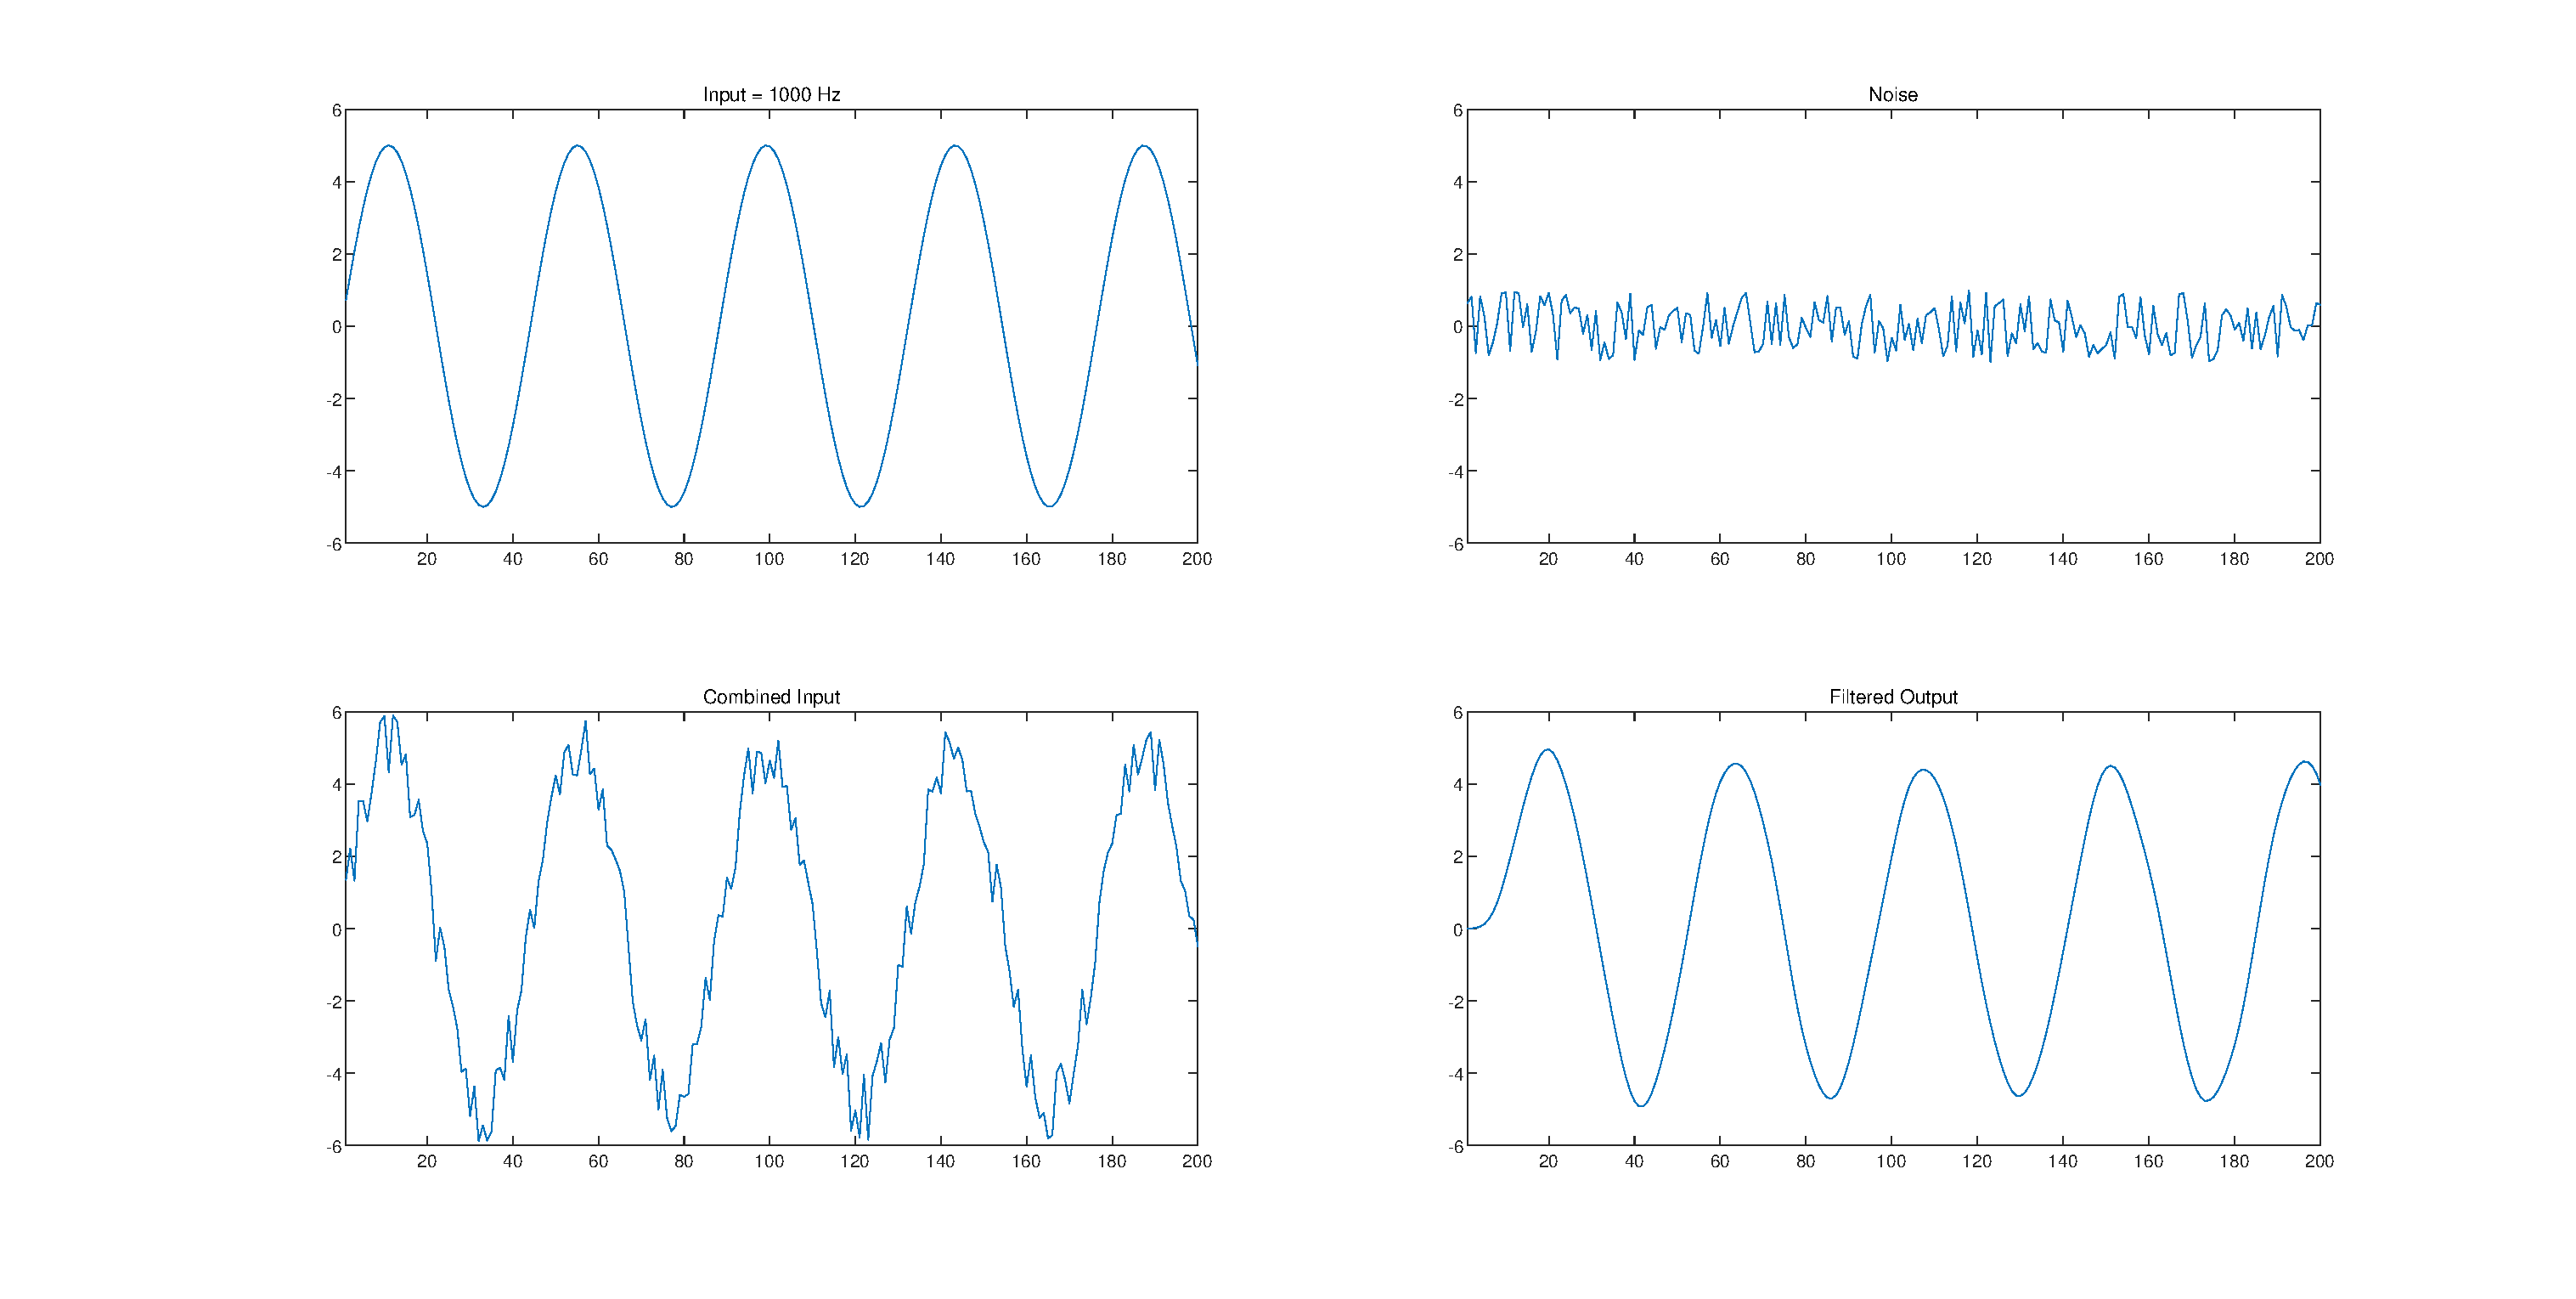
\includegraphics[width=0.8\textwidth]{images/mlhdlc_fir_tb_io_plot.eps}
    \caption{The input/output plot of the FIR filter.}
\end{figure}
\begin{figure}[H]
    \centering
    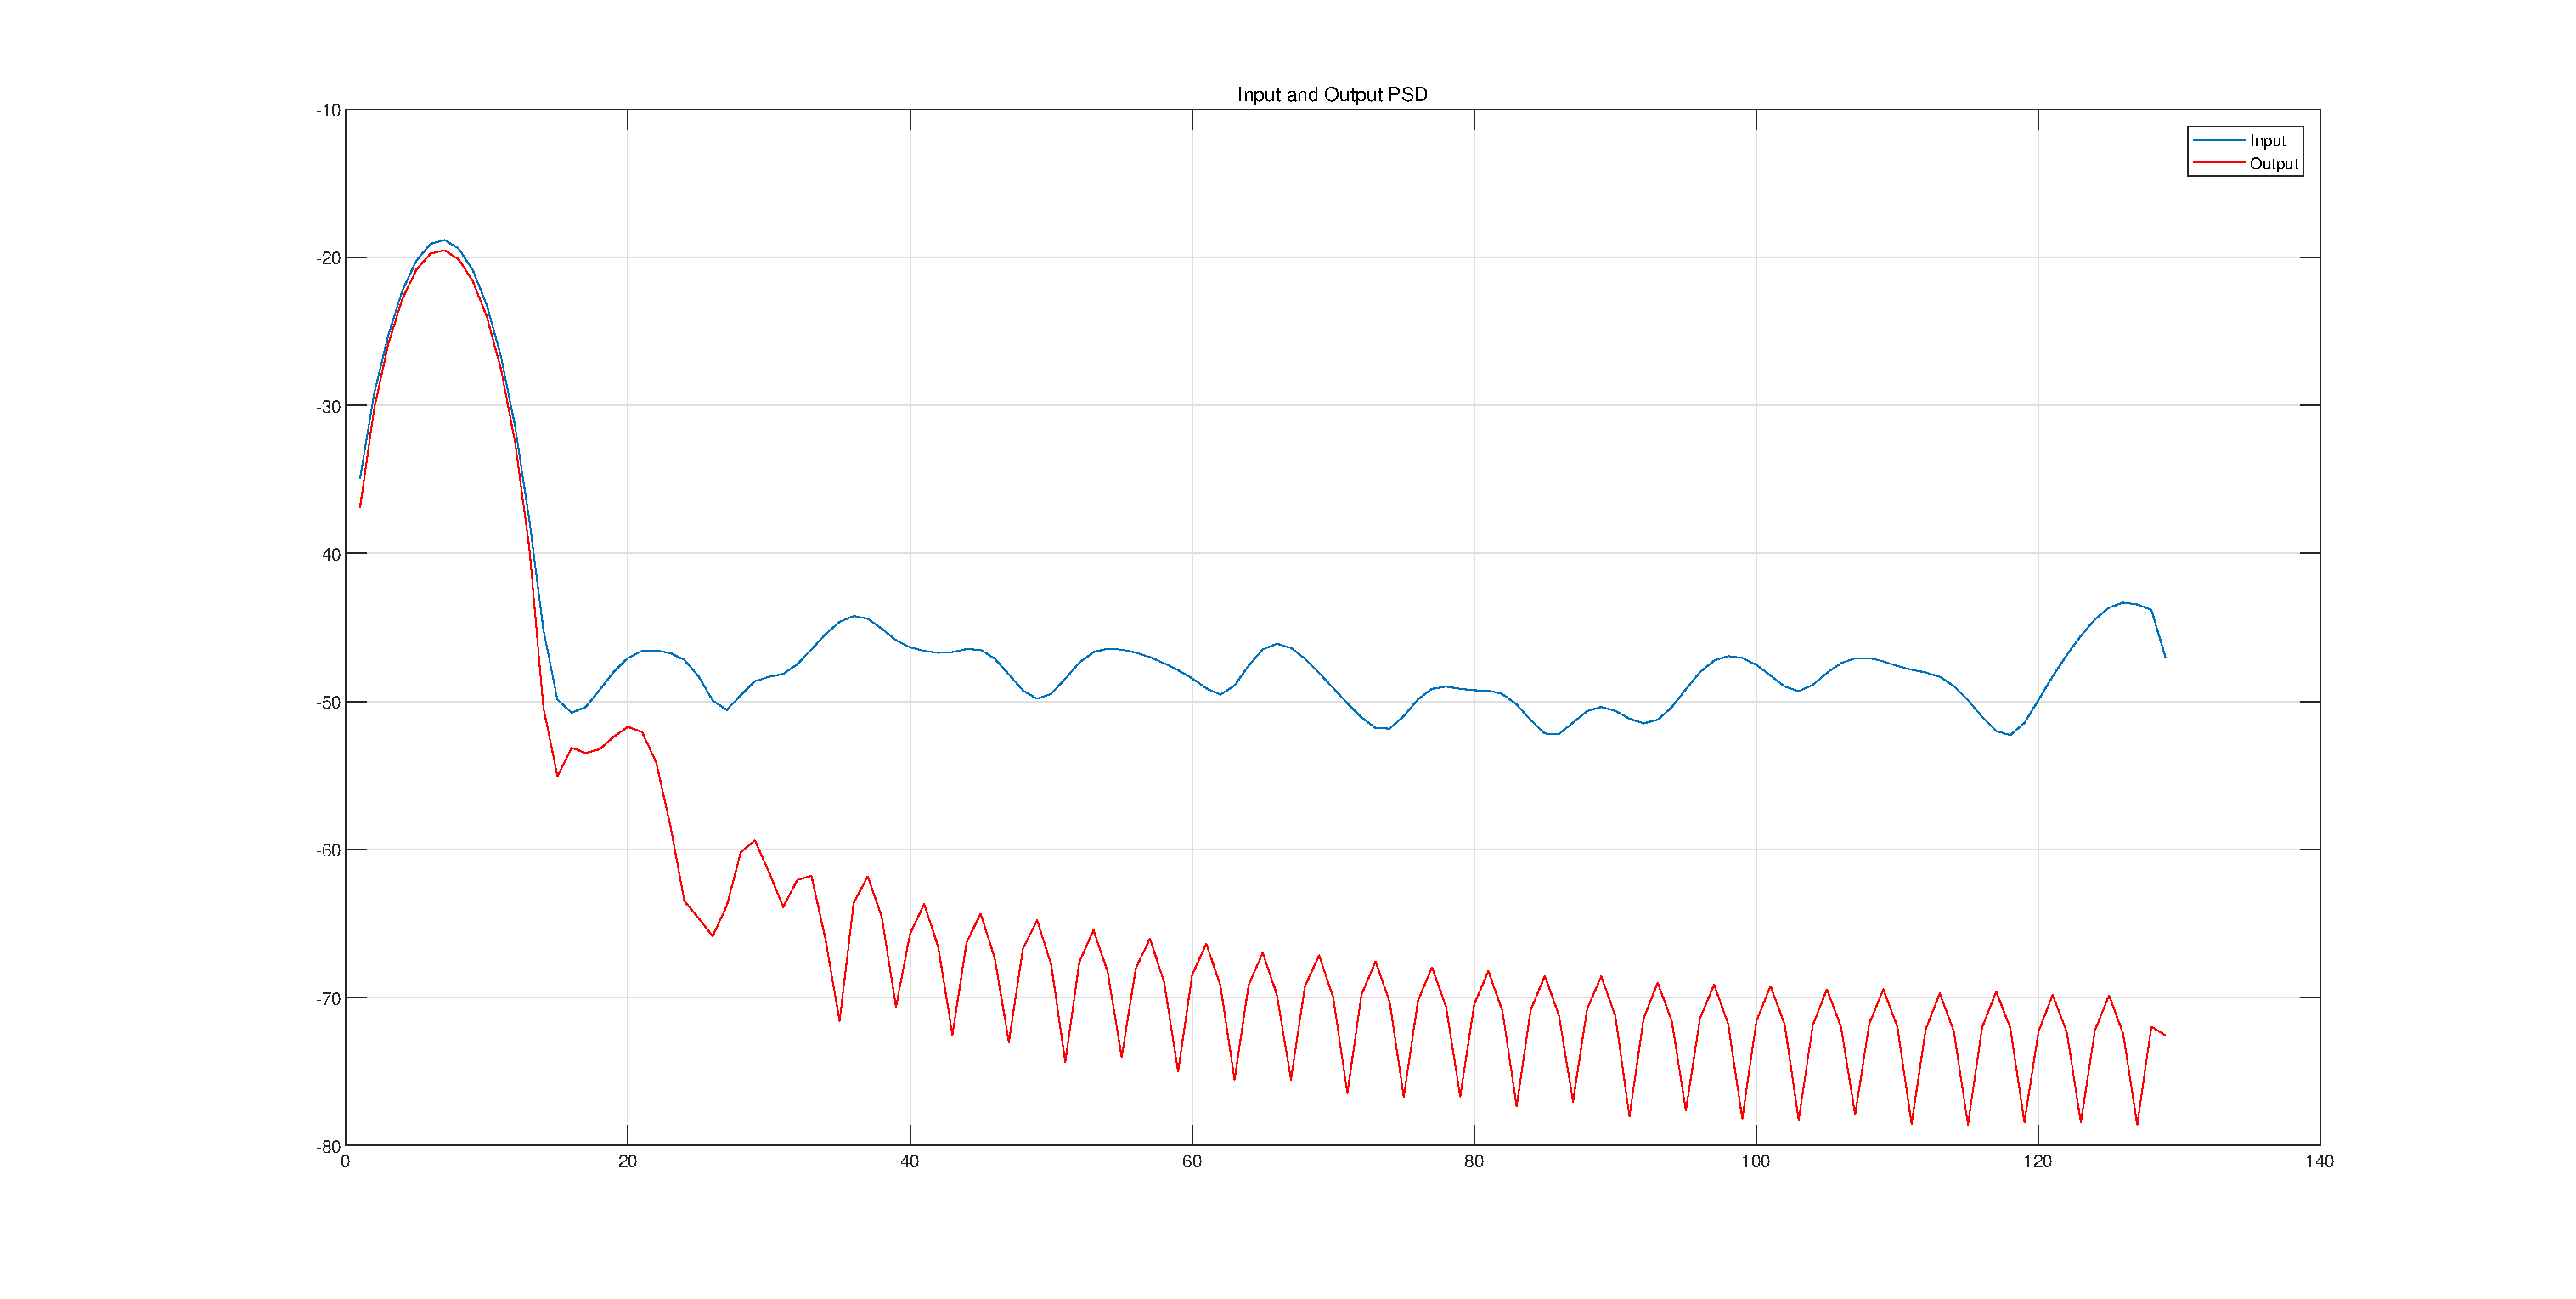
\includegraphics[width=\textwidth]{images/mlhdlc_fir_tb_psd_plot.eps}
    \caption{The power spectral density (PSD) plot of the FIR filter.}
\end{figure}
Run
\begin{minted}[breaklines,breakanywhere]{matlab}
hdlsetuptoolpath('ToolName','Xilinx Vivado','ToolPath','F:\Xilinx\Vivado\2022.1\bin\vivado.bat')
\end{minted}
to prepend the Xilinx Vivado path to the system path. Run
\begin{minted}{matlab}
coder -hdlcoder -new fir_project
\end{minted}
In the HDL Code Generation tab on the right, add MATLAB function \texttt{mlhdlc\_fir.m} and add \texttt{mlhdlc\_fir\_tb.m} as MATLAB Test Bench. Click "Autodefine types". In the pop-up dialog "Autodefine Input Types", select \texttt{mlhdlc\_fir\_tb.m} as the Test file, and run. Open the Workflow Advisor, and you can see "Define Input Types" is ticked. The \texttt{indatabuf} is defined as a double($1\times1$). Click "Use These Types". Right-click "Fixed-Point Conversion" and run this task, or click DATA COLLECTION->Analyze. The Build Log is
\begin{minted}{text}
Code generation successful.
\end{minted}
The Simulation Output is
\begin{minted}{text}
### Analyzing the design 'mlhdlc_fir'
### Analyzing the test bench(es) 'mlhdlc_fir_tb'
### Begin Floating Point Simulation (Instrumented)
### Floating Point Simulation Completed in 9.8445 sec(s)
### Elapsed Time:            11.2084 sec(s)
\end{minted}
The Type Validation Output is
\begin{minted}{text}
### Generating Type Proposal Report for 'mlhdlc_fir' mlhdlc_fir_report.html
### Generating Fixed Point MATLAB Code mlhdlc_fir_fixpt using Proposed Types
### Generating Fixed Point MATLAB Design Wrapper mlhdlc_fir_wrapper_fixpt
### Generating Mex file for ' mlhdlc_fir_wrapper_fixpt '
Code generation successful: View report
\end{minted}
The Variables tab is:
\begin{figure}[H]
    \centering
    \includegraphics[width=\textwidth]{images/29.png}
\end{figure}
Then, go to "Select Code Generation Target", and set the target device and synthesis tool. Choose workflow as Generic ASIC/FPGA. If the Synthesis tool is "No synthesis tool available on system path", then click Refresh list as long as you run the \texttt{hdlsetuptoolpath} command previously. Then, you should see "No synthesis tool specified". Select Xilinx Vivado. Select Zynq as Chip family, xc7z020 as the device, and clg400 as the package.

In "HDL Code Generation", generate synthesizable HDL code from the fixed-point MATLAB code. In the Target tab, for Target Selection, select Verilog. Check "Check HDL conformance", "Generate HDL", and "Generate EDA scripts". In the Coding Style tab, for Generated Code Comments, check "Preserve MATLAB code comments" and "Generate report". In the Optimizations tab, specify 1 for Input pipelining and Output pipelining, and then select Distribute pipeline registers. In the Advanced tab, check Generate MATLAB Function Block (Simulation license is required) from Simulation Integration. Click Run to generate Verilog code. Look through HDL Code Generation Check Report for 'mlhdlc\_fir\_fixpt'.
\begin{minted}[breaklines]{text}
### Begin Verilog Code Generation
### Working on mlhdlc_fir_fixpt as mlhdlc_fir_fixpt.v.
### The DUT requires an initial pipeline setup latency. Each output port experiences these additional delays.
### Output port 1: 2 cycles.
### Output port 2: 2 cycles.
### Generating Resource Utilization Report resource_report.html.
 ### Generating HDL Conformance Report mlhdlc_fir_fixpt_hdl_conformance_report.html.
### HDL Conformance check complete with 0 errors, 1 warnings, and 0 messages.
 ### Code generation successful: View report
### Elapsed Time: '         20.4480' sec(s)
\end{minted}
The summary of the HDL resource utilization report is
\begin{table}[H]
    \centering
    \begin{tabular}{|c|c|}
        \hline
        Multiplier & 16 \\
        \hline
        Adders/Subtractors & 31 \\
        \hline
        Registers & 19 \\
        \hline
        Total 1 Bit Registers & 253 \\
        \hline
        RAMs & 0 \\
        \hline
        Multiplexers & 0 \\
        \hline
        I/O Bits & 32 \\
        \hline
        Shifters & 0 \\
        \hline
    \end{tabular}
    \caption{The summary of HDL resource utilization report.}
\end{table}
\begin{figure}[H]
    \centering
    \includegraphics[width=\textwidth]{images/30.png}
    \caption{The MATLAB Function Block of FIR filter.}
\end{figure}
\subsection{Basic HDL Code Generation and FPGA Synthesis from MATLAB}
Now, your first task is to use mlhdlc\_sfir.m and mlhdlc\_sfir\_tb.m to finish the full workflow. Run
\begin{minted}{matlab}
coder -hdlcoder -new sfir_project
\end{minted}
Finish all steps mentioned before and save the mlhdlc\_sfir\_tb\_plot. Then in HDL Verification->Verify with HDL Test Bench, verify the HDL code with test vectors from the test bench using the specified simulation tool. In the Output Settings tab, from HDL Test Bench Generation Settings, check "Generate HDL test bench". If you have Mentor ModelSim installed, from HDL Test Bench Simulation Settings, check Simulate generated HDL test bench and select ModelSim as the Simulation tool. You can check the test bench data files and the compilation report mlhdlc\_sfir\_fixpt\_vsim\_log\_compile.txt, and the simulation report mlhdlc\_sfir\_fixpt\_vsim\_log\_sim.txt.

You can also generate and run a cosimulation test bench in Verify with Cosimulation. In the Output Settings tab, from Cosimulation Test Bench Generation Settings, check "Generate cosimulation test bench". If you have Mentor ModelSim installed, you can check Log outputs for comparison plots, choose Cosimulation for use with Mentor Graphics ModelSim, and select "GUI" for HDL simulator run mode in cosimulation. You may save the plot of y\_out difference and the plot of delayed\_xout difference, and take a screenshot of the waveform of all the In and Out signals in ModelSim. You can also check the Simulation generated cosimulation test bench from Cosimulation Test Bench Simulation Settings. The "cosim" directory is under mlhdlc\_sfir/codegen/mlhdlc\_sfir.

Unfortunately, Arty boards are not supported by MATLAB HDL Coder (including MathWorks HDL Coder Team's HDL Coder Support Package for Xilinx FPGA Boards and MathWorks HDLVerfier Team's HDL Verifier Support for Xilinx FPGA Boards) yet, so we have to skip "Verify with FPGA-in-the-Loop" that generates and runs FPGA-in-the-Loop test bench.

You can now directly do Synthesis and Analysis here by Xilinx Vivado. Create a synthesis project for the specified synthesis tool. You can see "Synthesis project creation successful". Then, go to "Run Synthesis" and run to synthesize and map the generated HDL code. You can check the synthesis report mlhdlc\_sfir\_fixpt\_syn\_results.txt and the parsed resource report file mlhdlc\_sfir\_fixpt\_utilization\_synth.rpt. Finally, go to "Run Implementation" and run to place and route (PAR) the generated HDL code for the specified hardware. You can check the parsed resource report file mlhdlc\_sfir\_fixpt\_utilization\_placed.rpt, and the parsed timing report file\\
timing\_post\_route.rpt.
\subsection{Generate HDL Code from Simulink Model}
In this subsection, you are going to reproduce the result of the article "Design and Comparison of FIR Filter Based on DSP Builder and HDL Coder" in \textit{2020 IEEE 15th International Conference on Solid-State \& Integrated Circuit Technology (ICSICT)} \cite{9278259}. Do not be panic. This article is so simple and low-quality that you may question how it could be selected for the conference.

Before working, you should be familiar with some concepts. The number of \textbf{tap}s of a filter = the filter length. The \textbf{order} of a filter is the number of non-zero taps of a filter. In the article, the number of taps is 16, but the constant term of a general 16-tap FIR filter is 0, so the order of the filter is 15 \cite{dspex}. The diagram for a common T-tap FIR filter is
\begin{figure}[H]
    \centering
    \includegraphics[width=\textwidth]{images/31.png}
    \caption{The diagram for a common T-tap FIR filter \cite{firan}.}
\end{figure}
Firstly, open the filter designer of MATLAB from the APP tab or run
\begin{minted}{matlab}
filterDesigner
\end{minted}
from the command line. Choose the direct I-type filter structure. Choose low-pass for Response type, FIR - Window for Design Method; specify 15 for Filter Order. In Options, choose Kaiser window with Beta = 0.5. In the Frequency Specifications frame, set Units = MHz, sampling frequency Fs = 12.5, cutoff frequency Fc = 2 \cite{firbeamer}.

Kaiser window or Kaiser–Bessel window and its Fourier transform is given by
\begin{equation}
w_0(x) \triangleq \left\{
\begin{array}{ccl}
\tfrac{1}{L}\frac{I_0\left[\pi\alpha \sqrt{1 - \left(2x/L\right)^2}\right]}{I_0[\pi\alpha]},\quad &\left|x\right| \leq L/2\\
0,\quad &\left|x\right| > L/2
\end{array}\right\}
\quad \stackrel{\mathcal{F}}{\Longleftrightarrow}\quad
\frac{\sin\bigg(\sqrt{(\pi L f)^2-(\pi \alpha)^2}\bigg)}
{I_0(\pi \alpha)\cdot \sqrt{(\pi L f)^2-(\pi \alpha)^2}}
\end{equation}
For digital signal processing, the function can be sampled symmetrically as:
\begin{equation}
    w[n] = L\cdot w_0\left(\tfrac{L}{N} (n-N/2)\right) = \frac{I_0\left[\pi\alpha \sqrt{1 - \left(\frac{2n}{N}-1\right)^2}\right]}{I_0[\pi\alpha]},\quad 0 \leq n \leq N
\end{equation}
The filter configuration is:
\begin{figure}[H]
    \centering
    \includegraphics[width=\textwidth]{images/full_view_analysis.eps}
    \caption{The filter configuration.}
\end{figure}
The visualization of the Kaiser window is
\begin{figure}[H]
    \centering
    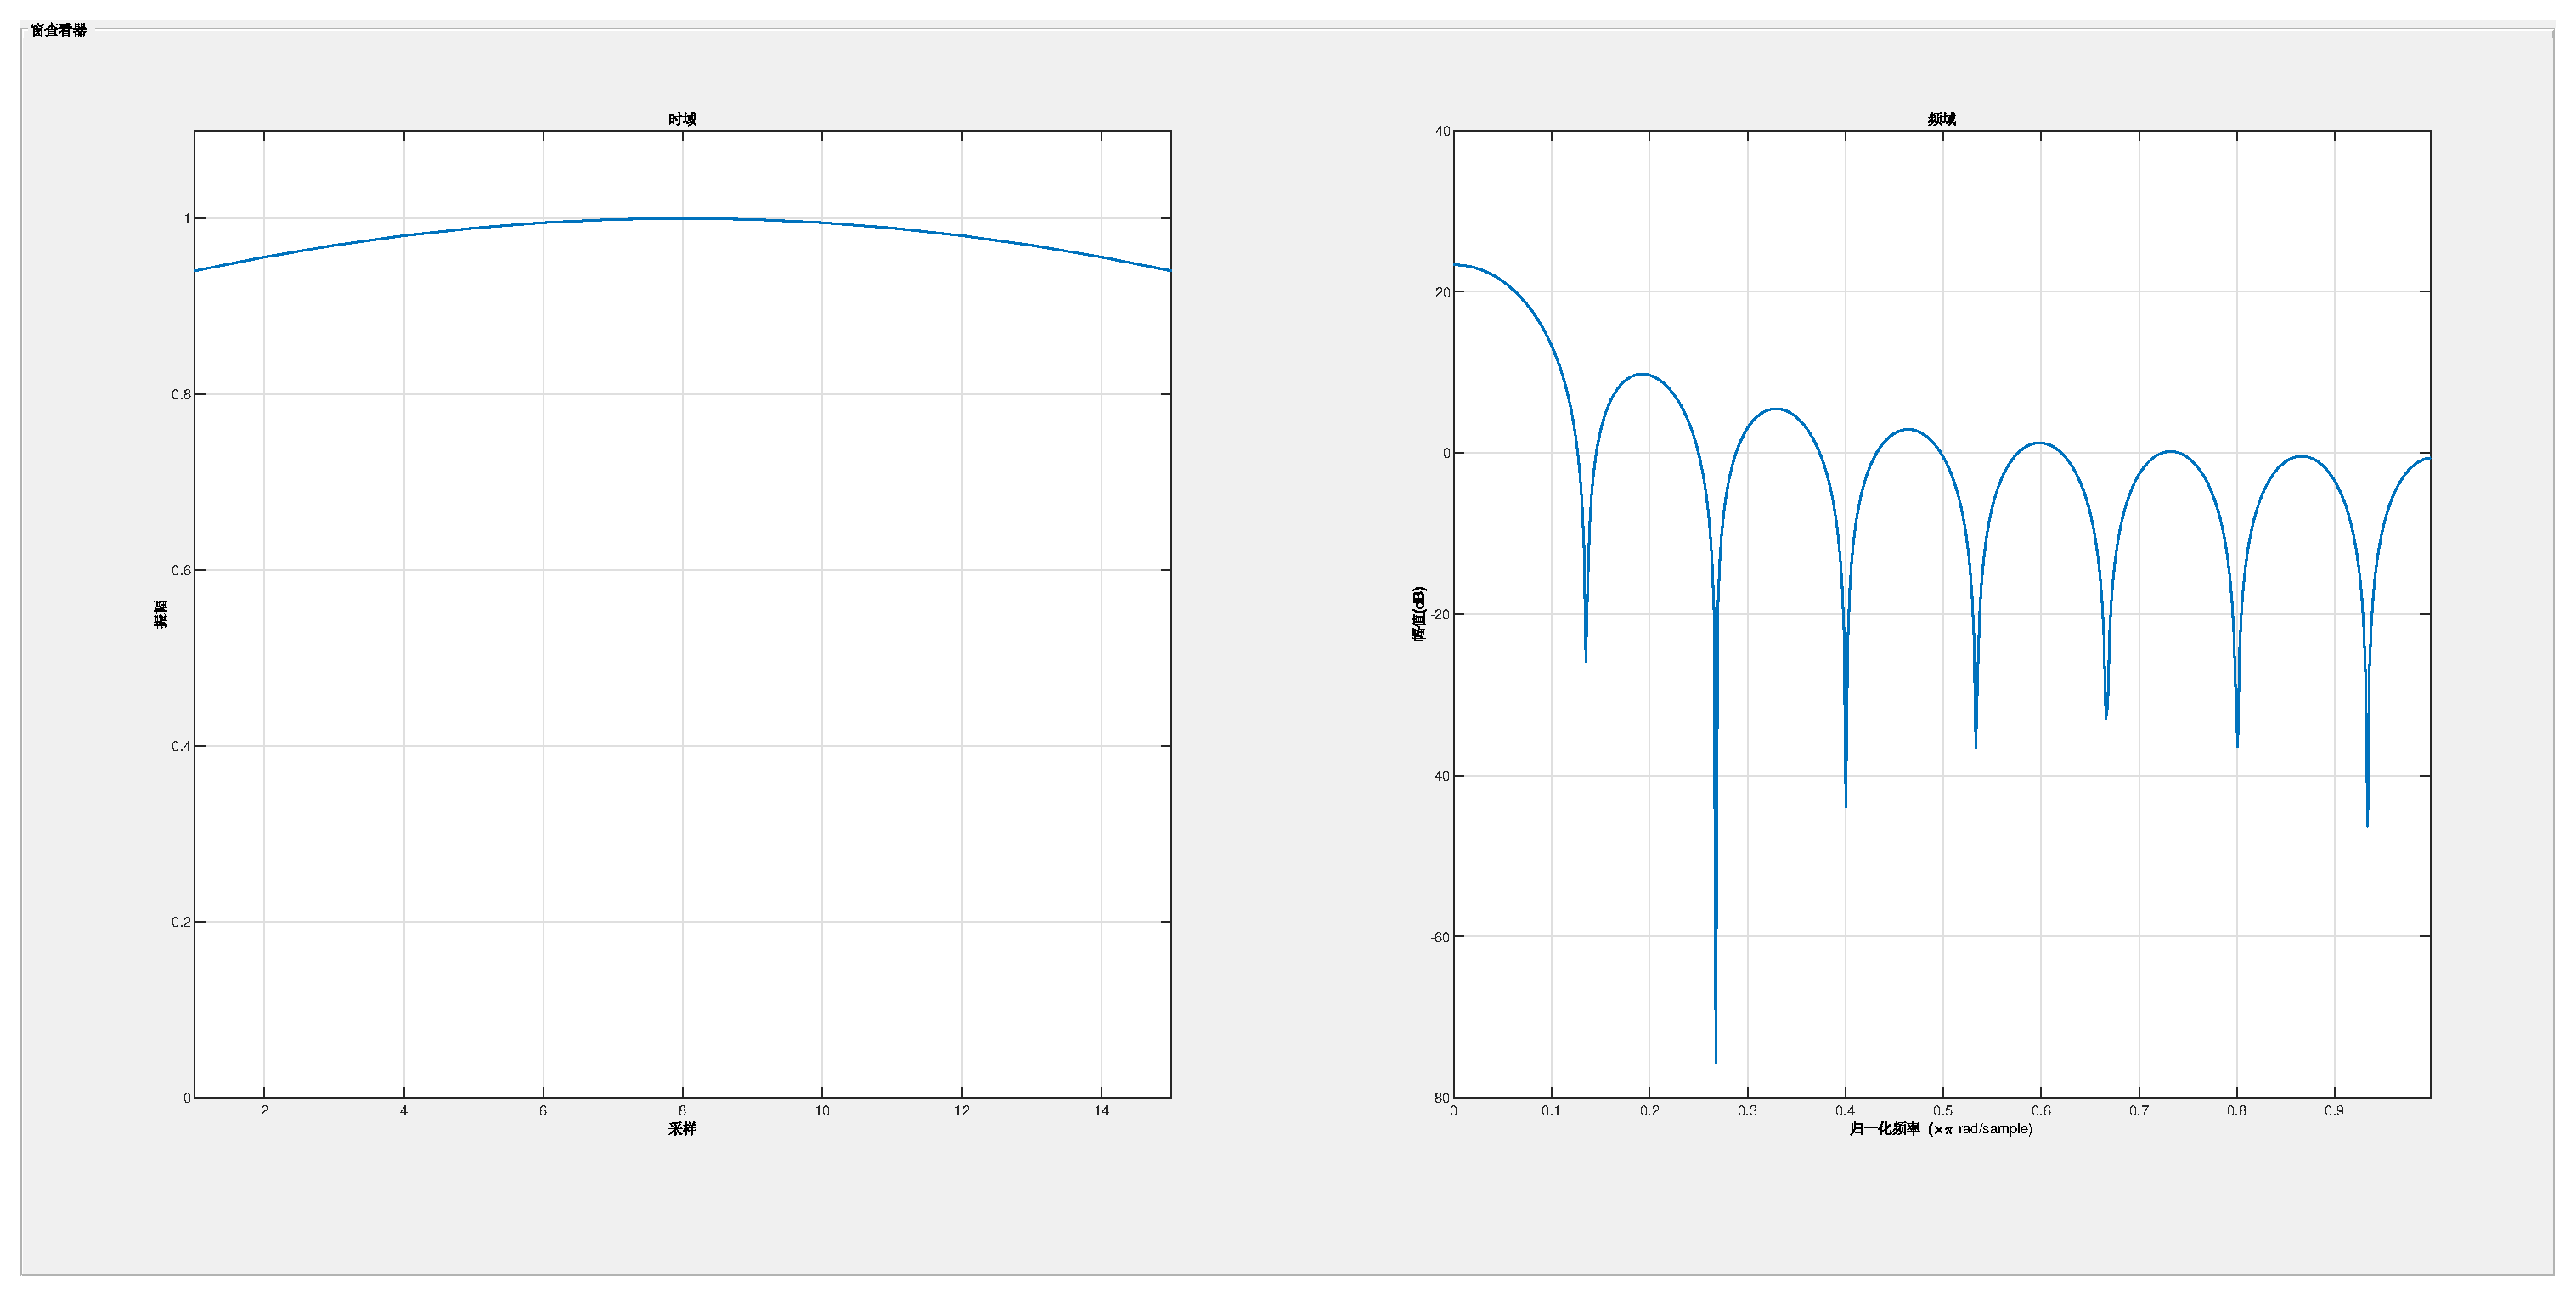
\includegraphics[width=\textwidth]{images/window_visualization_tool.eps}
    \caption{The visualization of the Kaiser window.}
\end{figure}
The frequency and phase response is
\begin{figure}[H]
    \centering
    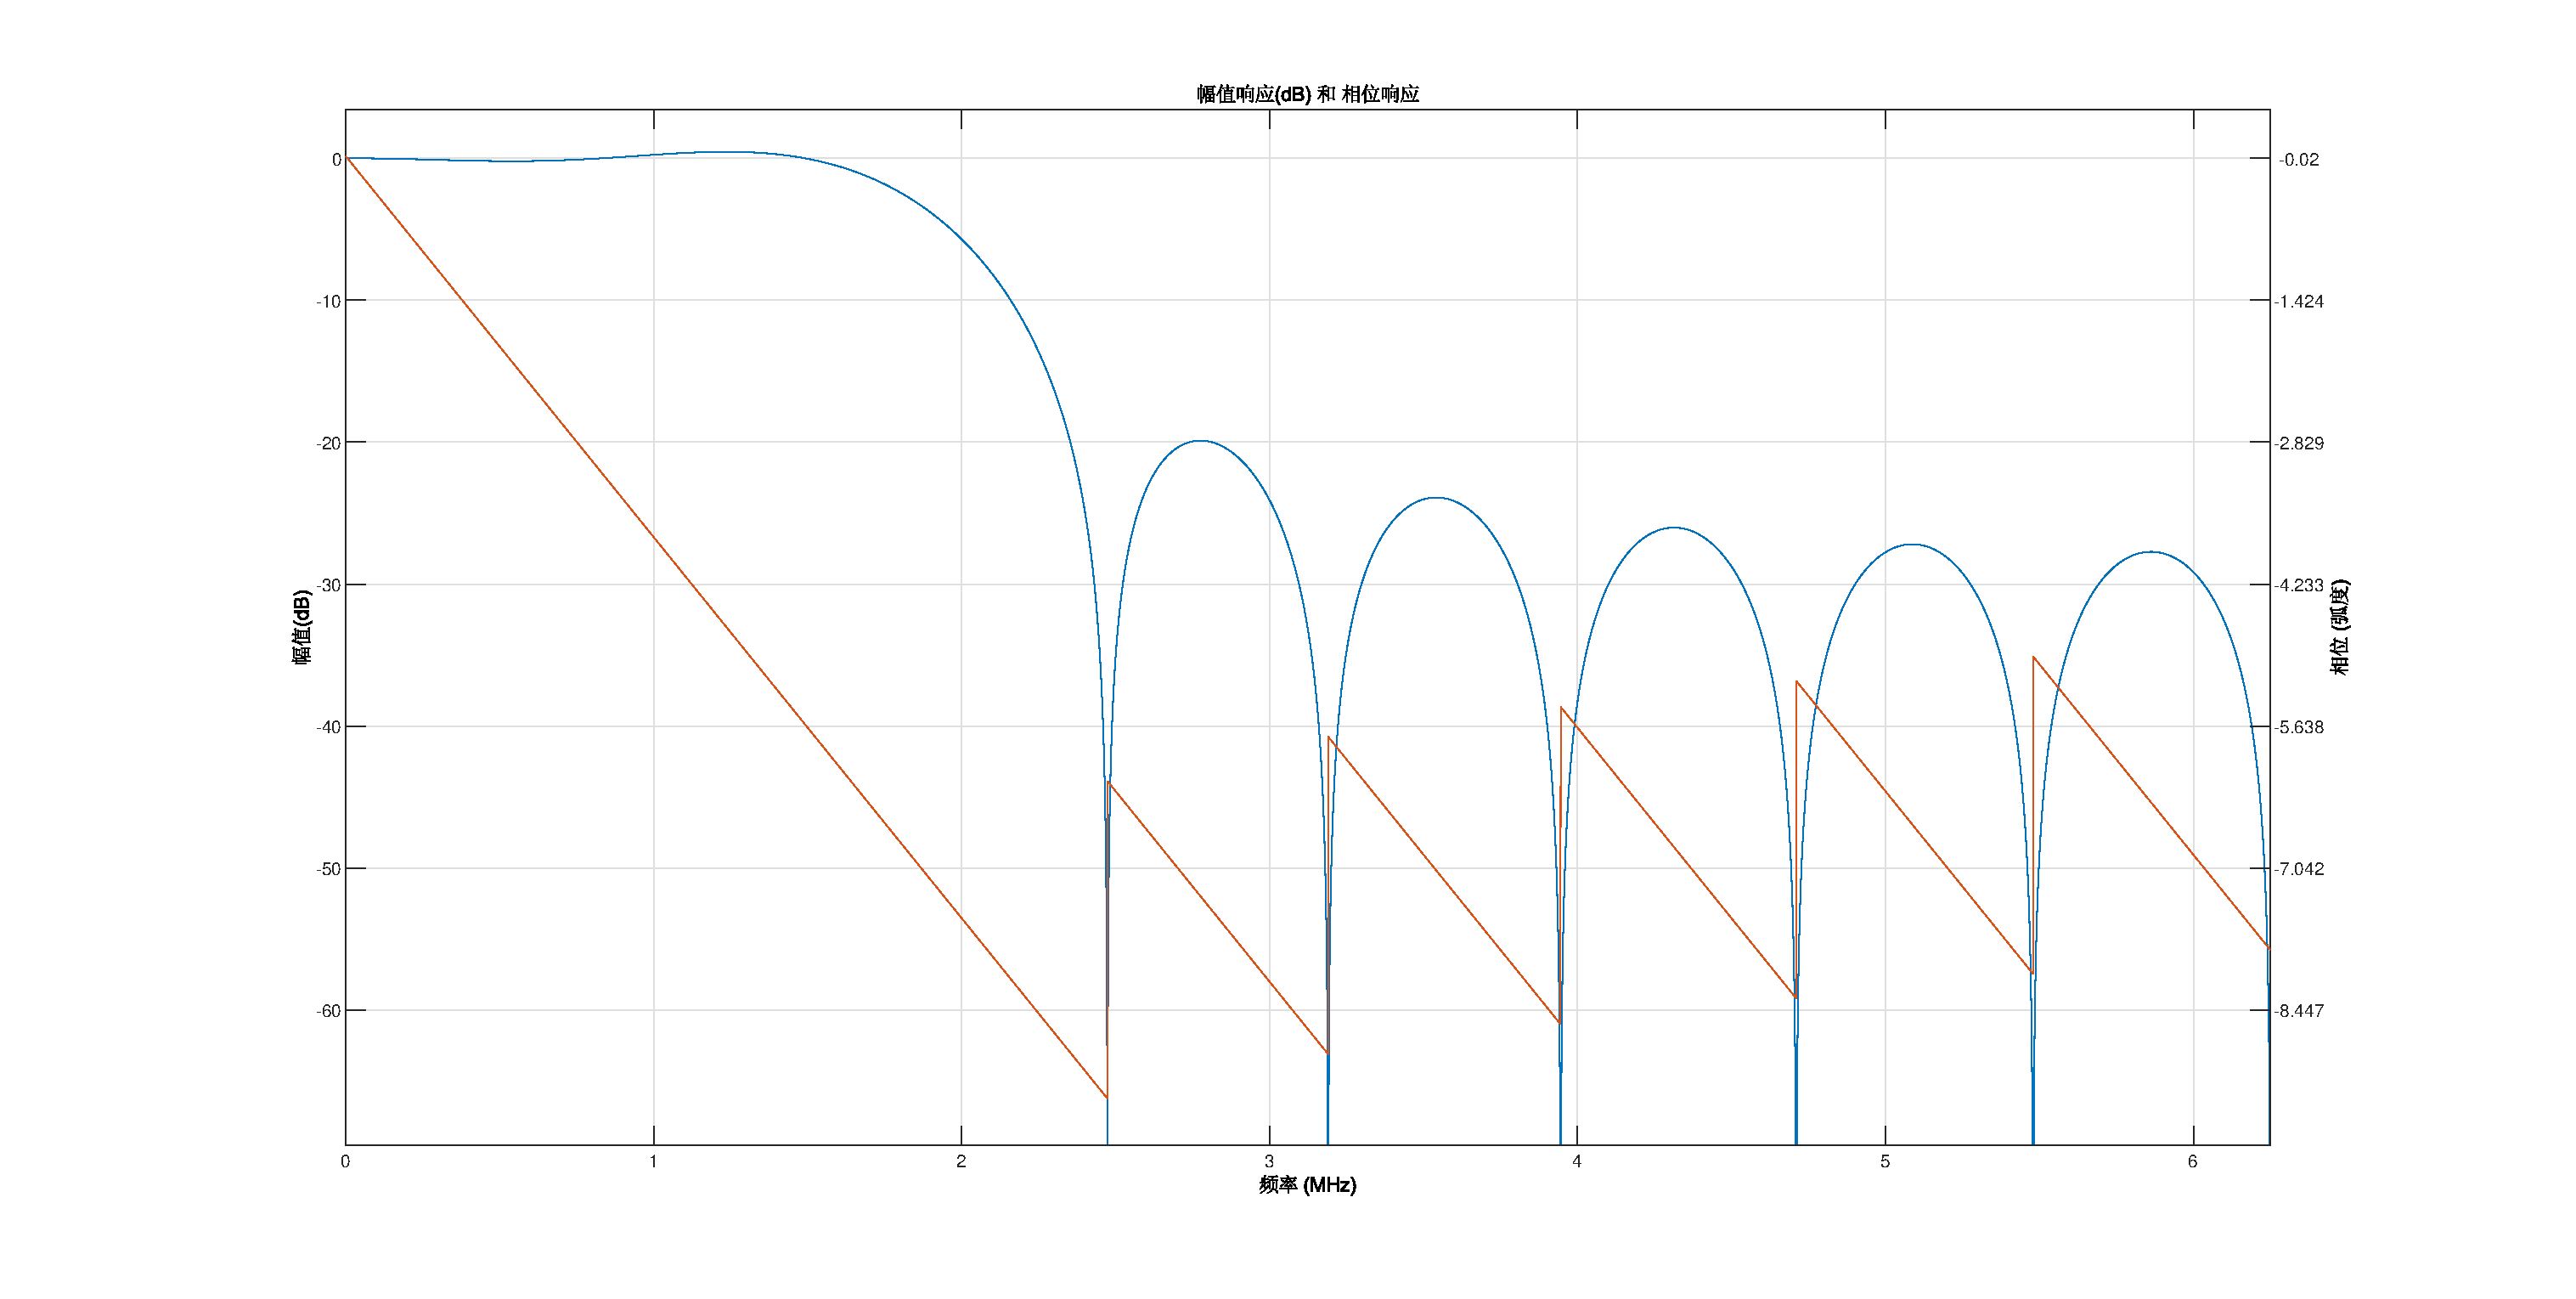
\includegraphics[width=\textwidth]{images/fvtool.eps}
    \caption{The frequency and phase response.}
\end{figure}
You can derive the filter coefficients from the filter designer. Note that the filter coefficients are symmetric.

Open Simulink. From HDL Coder, create a Blank DUT SLX. Feel free to refer to \cite{sleg}. Remember that only add components from the HDL Coder category in the library browser. To inspect the waveform, you can add a scope at the endpoint, but to generate HDL code, you must also add an Out1 from the Sinks category at the endpoint. Since the filter coefficients are symmetric, you can share one coefficient between a pair of delays. For \texttt{x\_in}, you can either use Sine Waves as the article uses or use the data From Workspace of a trigonometric function as Sources as MATLAB Documentation uses; for \texttt{h\_in}, use your previously generated filter coefficients, and you can serve them as Constant inputs or as the Gain by multiplication. If using Sine Waves, set Frequency (Hz) and Sample time to proper values. You can establish a model hierarchy that encapsulates your FIR filter into a DUT. Also, carefully set the (output) data types. If you set double, the simulation or code generation will fail because Sine Wave should be computed by Table lookup, and no floating point IP library is to be used, so you have to set by \texttt{fixdt}. \textit{Hint: you only need to specify the output data type of source modules explicitly, then Simulink will automatically determine the data type as Inherit: auto and the output data type as Inherit: Inherit via internal rule.} There are various valid data type configurations. Data Type Conversion module is allowed but is not necessary. To make a tidy output waveform, set the proper stop time of the simulation.

After the Simulink model is finished, in the App tab, open HDL Coder, then you can open the Workflow Advisor in the ASSISTANCE frame in the HDL CODE tab. This HDL Workflow Advisor is slightly simpler than what we used before. Set the target device, the synthesis tool, and the target frequency. Unfortunately, Xilinx Vivado Tool version 2022.1.2 is not supported yet, so you need to check "Allow unsupported version". Ignore the warning information:
\begin{minted}[breaklines]{text}
Warning Version 2022.1.2 of tool Xilinx Vivado is not supported in HDL Workflow Advisor. Using incompatible tool version, HDL Workflow Advisor may not be able to run further tasks. Attempting to continue using this tool version.
\end{minted}
\begin{figure}[H]
    \centering
    \includegraphics[width=\textwidth]{images/32.png}
\end{figure}
In Step 3: HDL Generation->3.1 Set HDL Options, click HDL Code Generation Settings... In the Set Basic Options frame, select Verilog as Language. In Floating Point->Floating Point IP Library, choose None. In Report->Optimization Reports, choose Generate resource utilization report and Generate optimization report. In Step 3.2: Generate RTL Code and Testbench, check all three input arguments. Run. You may need to modify your design if the run fails or the generated Verilog module is empty.

To run the simulation, you can right-click your Scope and press "P" to open the Scope window. Click the green button on the top of the Scope window or the Simulink window to run. In View->Configuration properties(C)... you can set 2 input ports; set automatic Coordinate scaling; in the Record tab, uncheck the first option to prevent limiting the data points to last. Enable legends. You can split the view of two wires into two views in View->Layout(L)... After the simulation is finished, compare the two views and take a screenshot. Your waveform does not need to be completely identical to the article's waveform, but you should write some sentences to explain your result in your report.

Run Step 4: FPGA Synthesis and Analysis. Ignore the warning:
\begin{minted}[breaklines]{text}
Warning Downstream Integration: Current version 2022.1.2 of Xilinx Vivado tool on system path may not be compatible with HDL Workflow Advisor. The compatible version: Xilinx Vivado 2020.2. Attempt to continue running Xilinx Vivado ...
\end{minted}
Take a screenshot of the Resource summary and the Timing summary of the implementation.

(Optional) If you have ModelSim installed, simulate the output Verilog HDL code. Take a screenshot of the waveform of the endpoint wires.

\newpage
\section{Tcl exercises}\label{STcl}
\subsection{Average}
Write a procedure (\texttt{proc}) called \texttt{avg} that takes an array of numbers with any length and returns the average of it.

Example:
\begin{minted}{tcl}
% puts [avg {70 80 50 60}]
65
\end{minted}
\subsection{Factorial}
Write a procedure (\texttt{proc}) that does the factorial function.

Example:
\begin{minted}{tcl}
% puts [factorial 3]
6
\end{minted}
\subsection{Two-fer}
Given a file name, return a string with messages. If given name, return "C source: main.c"; otherwise, return "C source:" and the given name.

Requirement:\\
Not allowed to use the keyword \texttt{args}. The body of the procedure should be one line.

Example:
\begin{minted}{tcl}
% two-fer
C source: main.c
% two-fer lab1-1.c
C source: lab1-1.c
\end{minted}
\section{Post-lab questions}\label{SQ}
Write short answers to the following questions:
\begin{enumerate}
    \item What is a bare metal test?
    \item How does the Zynq PS communicate with the IP blocks we created in this lab?
    \item Summarize the main features of AXI from the reading material
\end{enumerate}
\newpage
\section{Deliverables}
Group Deliverables (Compile everything as a single pdf report besides the code):
\begin{itemize}
    \item Section \ref{S2}: the screenshot of the Vitis IDE window in the build finished state and the screenshot of Vitis Serial Terminal
    \item Section \ref{S3}: the screenshot of the Implemented Design, including the Design Timing Summary of the Xilinx Vivado project, the screenshot of the Vitis IDE window in the build finished state, four photos of the board, and the code
    \item Section \ref{S4}: the resource utilization report/screenshot, the screenshot of the Vitis IDE window in the build finished state and the screenshot of Vitis Serial Terminal for both rtl\_multiplier and rtl\_divider
    \item Section \ref{Sopt1}.3 (optional): the mlhdlc\_sfir\_tb\_plot of the SFIR filter, the HDL resource utilization report of the SFIR filter, the MATLAB Function Block of the SFIR filter, the screenshot of the implementation design including the Design Timing Summary of the Vivado project mlhdlc\_sfir\_fixpt\_vivado.xpr;\\
    if applicable (not counted for grade), the plot of y\_out difference, the plot of delayed\_xout difference, mlhdlc\_sfir\_fixpt\_vsim\_log\_compile.txt,\\
    mlhdlc\_sfir\_fixpt\_vsim\_log\_sim.txt, and the screenshot of the waveform of all the In and Out signals in ModelSim
    \item Section \ref{Sopt1}.4 (optional): the Simulink model lab1\_3.slx file, your generated Verilog HDL code from Simulink, the screenshot of the Resource summary and the Timing summary of the implementation from Simulink
    \item Section \ref{STcl}: Tcl code
    \item Section \ref{SQ}: answer
\end{itemize}
Remember to add some comments or explanations on all the deliverables of Sections \ref{S2} - \ref{Sopt1} in your report.
\section{Grading policy}
\begin{table}[H]
    \centering
    \begin{tabular}{|c|c|}
        \hline
        Factors & Percentage \\
        \hline
        Section \ref{S2} & 12\% \\
        \hline
        Section \ref{S3} & 30\% \\
        \hline
        Section \ref{S4} & 40\% \\
        \hline
        Section \ref{Sopt1} & 20\% (bonus) \\
        \hline
        Section \ref{STcl} & 9\% \\
        \hline
        Section \ref{SQ} & 9\% \\
        \hline
    \end{tabular}
\end{table}
% The bonus points will be added to your grade of this lab.

\newpage
\appendix
\section{Peer Evaluation Form}
Each team member is required to provide a peer evaluation of the team effort of the lab. The score of the peer evaluation should be integers ranging between 0 to 5, inclusively, with 5 indicating the biggest contribution. A score should be given to each team member including yourself according to the team member’s contribution based on your observation. A brief
description of the contribution of each team member should also be provided, as shown in the following table.
\begin{table}[H]
    \centering
    \begin{tabular}{|c|c|c|c|c|}
        \hline
        Part & Your work & Your partner's work & Your score & Your partner's score \\
        \hline
        Section \ref{S2} & & & & \\
        \hline
        Section \ref{S3} & & & & \\
        \hline
        Section \ref{S4} & & & & \\
        \hline
        Section \ref{Sopt1} & & & & \\
        \hline
        Section \ref{STcl} & & & & \\
        \hline
        Section \ref{SQ} & & & & \\
        \hline
    \end{tabular}
\end{table}
Note that the score you give is not decisive. Your peer evaluation score may be adjusted according to your work described based on certain fair policies so that as long as your partner and you assume a similar workload, both of you can get full scores, but if the workload is very different though you and your partner give the identical scores, the scores will be adjusted. Your final lab grade may be scaled by the individual difference (the individual average divided by the group average). You cannot submit a peer evaluation form with the same contents as your partner's; otherwise, 3 points of deduction will be applied to your total grade for this lab.

\newpage
\section{Troubleshooting}
\subsection{Vivado Export Hardware}\label{AA1}
If you see error messages like
\begin{enumerate}
    \item {[BD 41-2008]} No default platform clock is selected. Please set property is\_default to true for one of the platform clocks
    \item {[Project 1-1038]} Failed to generate hpfm file for BD file:\\
    F:/Documents/GitHub/ECE4810J\_FA2022\_TA/Lab1/lab1\_1/lab1\_1.srcs/\\
    source\_1/bd/Zynq\_CPU/Zynq\_CPU.bd
    \item {[Common 17-53]} User Exception: Unable to get hpfm file from project property platform.hpfm\_file or from the BD itself
\end{enumerate}
\begin{figure}[H]
    \centering
    \includegraphics[width=0.65\textwidth]{images/17.png}
\end{figure}
Please see the reference article \cite{vivadoexport}.
\subsection{Launch Xilinx Vitis}\label{AA2}
If Vitis fails to start up or does not respond at start-up, close Vivado and manually launch Vitis from your desktop or Start Menu \cite{vitis1}.
If you are prompted to install Microsoft Visual C++ 2015-2019 Redistributable (x64) - 14.29.30133, you will fail \cite{vivadotcl}.
\begin{figure}[H]
    \centering
    \includegraphics[width=0.5\textwidth]{images/10.png}
\end{figure}
You can just run Xilinx Vitis as administrator. If the menu of shortcut of Vitis has no "Run as Administrator", your shortcut probably points to\\ \texttt{F:\textbackslash Xilinx\textbackslash Vitis\textbackslash 2022.1\textbackslash bin\textbackslash vitis.vbs} file under your Vitis installation directory. There are some tricks you can find on Google about running VBS as administrator, but you would better run \texttt{F:\textbackslash Xilinx\textbackslash Vitis\textbackslash 2022.1\textbackslash bin\textbackslash vitis.bat} as administrator.

If Vitis still does not respond at start-up, use a text editor to edit \texttt{vitis.bat} file \cite{vitisrespond},
\begin{figure}[H]
    \centering
    \includegraphics[width=\textwidth]{images/11.png}
\end{figure}
add
\begin{minted}[breaklines,breakanywhere]{bat}
set PATH=
\end{minted}
to avoid PATH overflow \cite{vitis2}. After this is done, re-run \texttt{vitis.bat} as administrator, then everything should work.

To make start-up easier, you can create a shortcut of \texttt{vitis.bat}, change the icon as\\ \verb|F:\Xilinx\Vitis/2022.1\doc\images\ide_icon.ico|; click Advance (D)..., check run as administrator:
\begin{figure}[H]
     \centering
     \begin{subfigure}[b]{0.45\textwidth}
         \centering
         \includegraphics[width=\textwidth]{images/12.png}
     \end{subfigure}
     \hfill
     \begin{subfigure}[b]{0.45\textwidth}
         \centering
         \includegraphics[width=\textwidth]{images/13.png}
     \end{subfigure}
\end{figure}
Change the name to "Xilinx Vitis 2022.1" and substitute the original shortcut with it.
\subsection{Vitis Build}\label{AA3}
If you see a Warning window showing:
\begin{minted}[breaklines,breakanywhere]{text}
Executables selected for download on to the following processors doesn‘t exist or incorrectly specified. Do you wish to ignore them and proceed?
1. ps7_cortexa9_0
\end{minted}
\begin{figure}[H]
    \centering
    \includegraphics[width=\textwidth]{images/16.png}
\end{figure}
It means that you forgot to build the project before you ran it. Click "Build Project" in the "Project" menu \cite{vitisbuild}.

If you create the application project from the Empty Application(C) template for Section \ref{S4}, you will not include \texttt{platform.h} and will get ten errors:
\begin{minted}[breaklines,breakanywhere,linenos]{text}
../src/lab1-3.c:1:10: fatal error: platform.h: No such file or directory
    1 | #include "platform.h"
      |          \^~~~~~~~~~~~
compilation terminated.
make[1]: *** [src/subdir.mk:23: src/lab1-3.o] Error 1
make: *** [Makefile:18: all] Error 2
make: *** [Makefile:30: zynq_fsbl_bsp/ps7_cortexa9_0/lib/libxil.a] Error 2
make: *** [makefile:34: all] Error 2
make[1]: *** [Makefile:18: all] Error 2
make[1]: *** [Makefile:46: ps7_cortexa9_0/libsrc/rtl_multiplier_v1_0/src/make.libs] Error 2
make[1]: *** [src/subdir.mk:23: src/lab1-3.o] Error 1
make[2]: *** [Makefile:18: libs] Error 1
make[2]: *** [Makefile:46: ps7_cortexa9_0/libsrc/rtl_multiplier_v1_0/src/make.libs] Error 2
make[3]: *** [Makefile:18: libs] Error 1
\end{minted}
If your process of the building failed with:
\begin{minted}[breaklines,breakanywhere,linenos]{text}
"Compiling rtl_multiplier..."

cc1.exe: fatal error: *.c: Invalid argument
compilation terminated.
make[2]: *** [Makefile:18: libs] Error 1
make[1]: *** [Makefile:46: ps7_cortexa9_0/libsrc/rtl_multiplier_v1_0/src/make.libs] Error 2
make: *** [Makefile:18: all] Error 2
make: Leaving directory 'F:/Documents/GitHub/ECE4810J_FA2022_TA/Lab1/lab1_1/Zynq_CPU_wrapper_hw_platform_3/zynq_fsbl/zynq_fsbl_
bsp'
\end{minted}
\begin{minted}[breaklines,breakanywhere,linenos]{text}
"Compiling rtl_multiplier..."

cc1.exe: fatal error: *.c: Invalid argument
compilation terminated.
make[3]: *** [Makefile:18: libs] Error 1
make[2]: *** [Makefile:46: ps7_cortexa9_0/libsrc/rtl_multiplier_v1_0/src/make.libs] Error 2
make[1]: *** [Makefile:18: all] Error 2
make[1]: Leaving directory 'F:/Documents/GitHub/ECE4810J_FA2022_TA/Lab1/lab1_1/Zynq_CPU_wrapper_hw_platform_3/zynq_fsbl/zynq_fs
bl_bsp'

make: *** [Makefile:30: zynq_fsbl_bsp/ps7_cortexa9_0/lib/libxil.a] Error 2
\end{minted}
\begin{minted}[breaklines,breakanywhere,linenos]{text}
../src/lab1-3.c:2:10: fatal error: xbasic_types.h: No such file or directory
    2 | #include "xbasic_types.h"
      |          ^~~~~~~~~~~~~~~~
compilation terminated.
make[1]: *** [src/subdir.mk:26: src/lab1-3.o] Error 1
make: *** [makefile:34: all] Error 2
\end{minted}
you can see that \texttt{xbasic\_types.h} can be found under\\
\verb|Zynq_CPU_wrapper_hw_platform_3\zynq_fsbl\zynq_fsbl_bsp\ps7_cortexa9_0\include|. This is an old bug of Xilinx Vitis. Please read the reference article \cite{vitisgcc}.
\subsection{Vitis Program Device}\label{AA4}
Firstly, you need to check the connection between your computer and the Arty-Z7. If the connection is set up, then open "XSCT Console" in the "Xilinx" menu. Run command \cite{vitisprogram}
\begin{minted}{text}
xsct% connect
\end{minted}
\begin{figure}[H]
    \centering
    \includegraphics[width=\textwidth]{images/18.png}
\end{figure}
Then, it will show:
\begin{minted}{text}
Cannot create listening port tcp:127.0.0.1:3121: Socket bind error.
\end{minted}

You can refer to \cite{vitissocket}. In a nutshell, if you are using Windows, just run the command in the Command Line Prompt:
\begin{minted}{bat}
net stop winnat
\end{minted}
This command stops the Windows NAT Driver service. This service is required for the network communication of virtual machines like Windows Subsystem for Linux (WSL), so if you stop it, you will have problems with that. Restarting the computer will reset the configuration.

If you get an "Error Launching Program" window showing
\begin{minted}{text}
Error while launching program:

Memory write error at 0x100000. MMU section translation fault
\end{minted}
Please read the reference article: \cite{vitisarty}.
\subsection{AXI IP Connection}\label{AA5}
If Vivado fails to correctly assign addresses to each AXI IP connected to your processor, the Address Editor can be accessed through its tab in the Diagram pane. Addresses can be assigned to unmapped peripherals by typing the desired address into the peripheral's Master Base Address column. It should be noted that addresses must be aligned in the memory space - for instance, an address with a range of 4K (bytes) takes up a range of 0x1000 addresses and must have three trailing zeros. Address ranges for different segments cannot overlap. Assigning a segment to address 0 may result in assertions in some software drivers and should be avoided. After manually assigning addresses, the block design should be re-validated.
\begin{figure}[H]
    \centering
    \includegraphics[width=\textwidth]{images/21.png}
\end{figure}
\subsection{Vivado Startup}\label{AA6}
If Vivado is stuck initializing language server, in Tools -> Settings -> Tool Settings -> Text Editor -> Syntax Checking, change Syntax checking from Sigasi to Vivado \cite{vivadostart}:
\begin{figure}[H]
    \centering
    \includegraphics[width=\textwidth]{images/22.png}
\end{figure}

\printbibliography
\end{document}

